\documentclass{report}

% ==============================

% Configuration files for custom packages and macros
\input{config/preamble}
\input{config/macros}
\input{config/letterfonts}

% ==============================

\title{\Huge{COMP 458/558}\\Quantum Computing Algorithms}
\author{\huge{Micah Kepe}}
\date{}

% ==============================

\makeindex[title=Appendix, intoc]

% ==============================

\begin{document}

\maketitle
\newpage

% Add a blank page after the title
\null\thispagestyle{empty}
\newpage

% ==============================
% PREFACE
% ==============================
\chapter*{Preface}
Quantum computing is an emerging field poised to revolutionize multiple
disciplines, including cryptography, optimization, machine learning, and
scientific simulations. This handbook serves as a structured compilation of
notes from \textit{COMP 458/558: Quantum Computing Algorithms}, offered at Rice
University during Spring 2025. The content is derived from lectures,
discussions, and supplementary readings throughout the semester, aiming to
reinforce core concepts and provide a comprehensive reference for students
and enthusiasts alike.

\vspace{0.3cm}

\noindent
The notes begin with foundational mathematical principles, including linear
algebra and probability theory. Subsequent sections explore quantum circuits,
essential quantum gates, multi-qubit systems, and fundamental quantum
algorithms such as Grover’s search and Shor’s factoring algorithm. The latter
phases of the handbook introduce advanced topics, including variational
quantum algorithms, quantum simulation techniques, and emerging paradigms in
quantum machine learning and optimization.

\vspace{0.3cm}

\noindent
I would like to extend my deepest gratitude to \textbf{Professor Tirthak Patel},
whose guidance and expertise have been instrumental in shaping my
understanding of quantum computing. I am also grateful to my peers for the
collaborative discussions that enriched my learning experience.

\vspace{0.3cm}

\noindent
As quantum computing continues to evolve, these notes will remain a living
document, subject to refinement and expansion. I welcome feedback,
corrections, and contributions from readers to ensure the accuracy and
completeness of this resource.

\vspace{1cm}

\noindent \textbf{Micah Kepe}  \\
Rice University  \\
Spring 2025



% ==============================
% TABLE OF CONTENTS
% ==============================
\renewcommand*\contentsname{Table of Contents}
\pdfbookmark[section]{\contentsname}{toc}
\tableofcontents
\pagebreak

\clearpage
\pagenumbering{arabic}  % Switch back to Arabic numerals
\setcounter{page}{1}    % Reset page numbering


% ==============================
% START OF CONTENT
% ==============================

% ==============================
% PHASE I: INTRODUCTION
% ==============================
\chapter{Phase I: Introduction and Background}

% ● Overview of quantum computing concepts and
% applications
% ● Historical background and current state of quantum
% computing
% ● Review of linear algebra concepts, notation, and
% vector spaces
\section{Lecture 1: Overview of Quantum Computing Concepts}\label{sec:lecture1}
\dfn{Quantum Computing}{\textbf{Quantum computing} is a computational paradigm
  leveraging quantum mechanical principles such as superposition, entanglement,
  and interference to perform computations that can surpass the capabilities of
  classical systems for specific tasks.

  \footnote{Superposition \index{superposition} allows quantum bits (qubits)
    to exist in multiple states simultaneously, and entanglement enables
correlations between qubits even at a distance.}}

\subsection*{Historical Development of Quantum Computing}
\begin{itemize}
  \item \textbf{1980s-1990s:} Conception of quantum computing, with
    foundational ideas like the quantum Turing machine and quantum gates.

  \item \textbf{1990s-2000s:} Demonstration of key building blocks, such as
    quantum algorithms (e.g., Shor's and Grover's algorithms).

  \item \textbf{2016:} Emergence of quantum computing clouds, enabling
    access to quantum hardware via the internet.

  \item \textbf{2019:} First claims of \textbf{quantum advantage},
    showcasing tasks where quantum computers outperform classical
    counterparts.

  \item \textbf{2024:} Increasing qubit counts and improvements in quantum
    error correction techniques.

\end{itemize}

\subsection*{Applications of Quantum Computing}

Quantum computing offers \textbf{speedup} in areas such as:

\begin{enumerate}
  \item \textbf{Quantum Simulation:} Applications in chemistry, physics,
    and materials science, such as simulating molecular energy levels and
    drug discovery.

  \item \textbf{Security and Encryption:} Developing quantum-safe
    cryptographic protocols and random number generation.

  \item \textbf{Search and Optimization:} Enhancing solutions for weather
    forecasting, financial modeling, traffic planning, and resource
    allocation.

\end{enumerate}

\ex{Example: Quantum Speedup in Drug Discovery}{Drug discovery benefits from
  quantum simulation by enabling more accurate modeling of molecular
interactions, which classical computers struggle to achieve efficiently.}

\subsection*{Classical vs. Quantum Computing Paradigms}
\begin{itemize}

  \item \textbf{Classical Computing:\index{classical computing}} Utilizes
    traditional processing units (CPU, GPU, FPGA) and executes deterministic
    computations.

  \item \textbf{Quantum Computing:} Employs quantum processing units (QPU)
    with probabilistic computation based on quantum states.

\end{itemize}

\nt{Note: Classical computing paradigms still dominate in tasks that require
  precision and deterministic results. Quantum computing excels in
probabilistic or exponentially large state-space problems.}


\section{Lecture 2: Review of Linear Algebra Concepts}
\dfn{Vectors: Row and Column Vectors}{A \textbf{vector} is an ordered list of numbers, which can be represented as either a row or column vector. The components of vectors in quantum computing belong to the field of complex numbers ($\mathbb{C}$).}

\subsection*{Column Vectors}
A column vector is a vertical arrangement of numbers:
\[ \mathbf{v} = \begin{bmatrix} v_1 \\ v_2 \\ \vdots \\ v_n \end{bmatrix}, \quad v_i \in \mathbb{C}. \]

\subsection*{Row Vectors}
A row vector is the complex conjugate transpose (adjoint) of a column vector:
\[ \mathbf{v}^\dagger = \begin{bmatrix} \overline{v_1} & \overline{v_2} & \dots & \overline{v_n} \end{bmatrix}. \]

\dfn{Inner Product}{The \textbf{inner product} of two vectors $\mathbf{v}, \mathbf{w} \in \mathbb{C}^n$ is defined as:
\[ \langle \mathbf{v}, \mathbf{w} \rangle = \mathbf{v}^\dagger \mathbf{w} = \sum_{i=1}^n \overline{v_i}w_i. \]}

\ex{Example: Inner Product}{Let $\mathbf{v} = \begin{bmatrix} 1 + i \\ 2 \end{bmatrix}$ and $\mathbf{w} = \begin{bmatrix} 3 \\ i \end{bmatrix}$. Then:
\[ \langle \mathbf{v}, \mathbf{w} \rangle = (1 - i)(3) + (2)(i) = 3 - 3i + 2i = 3 - i. \]}

\dfn{Outer Product}{The \textbf{outer product} of two vectors $\mathbf{v} \in \mathbb{C}^m$ and $\mathbf{w} \in \mathbb{C}^n$ produces an $m \times n$ matrix:
\[ \mathbf{v}\mathbf{w}^\dagger = \begin{bmatrix} v_1 \\ v_2 \\ \vdots \\ v_m \end{bmatrix} \begin{bmatrix} \overline{w_1} & \overline{w_2} & \dots & \overline{w_n} \end{bmatrix}. \]}

\dfn{Orthogonality}{Two vectors $\mathbf{v}, \mathbf{w} \in \mathbb{C}^n$ are \textbf{orthogonal} if their inner product is zero:
\[ \langle \mathbf{v}, \mathbf{w} \rangle = 0. \]}

\ex{Example: Orthogonality}{Let $\mathbf{v} = \begin{bmatrix} 1 \\ i \end{bmatrix}$ and $\mathbf{w} = \begin{bmatrix} i \\ 1 \end{bmatrix}$. Then:
\[ \langle \mathbf{v}, \mathbf{w} \rangle = (1)(i) + (i)(1) = i - i = 0. \]}

\dfn{Eigenvalues and Eigenvectors}{For a square matrix $A \in \mathbb{C}^{n \times n}$, a vector $\mathbf{v} \neq \mathbf{0}$ is an \textbf{eigenvector} if:
\[ A\mathbf{v} = \lambda\mathbf{v}, \]
where $\lambda \in \mathbb{C}$ is the \textbf{eigenvalue}.}


%%%%

% ● Quantum state representation and quantum bits (qubits)
% ● Probability theory and its application to quantum systems
% ● Measurement and quantum state collapse
% ● Statistical analysis of quantum measurements
\section{Lecture 3: Quantum Bits and Quantum States}

\dfn{Qubit}{A \textbf{qubit} is the fundamental unit of quantum information. Unlike a classical bit, which is either $0$ or $1$, a qubit can exist in a \vocab{superposition} of states:
\[ |\psi\rangle = \alpha|0\rangle + \beta|1\rangle, \quad \text{where } \alpha, \beta \in \mathbb{C} \text{ and } |\alpha|^2 + |\beta|^2 = 1 \]

Key features of qubits include:
\begin{itemize}
    \ii \textbf{Superposition:} A qubit can exist simultaneously in multiple basis states.
    \ii \textbf{Complex Amplitudes:} Coefficients $\alpha$ and $\beta$ are complex numbers carrying magnitude and phase information.
    \ii \textbf{Interference:} Quantum states can interfere constructively or destructively.
    \ii \textbf{Entanglement:} Qubits can be correlated in ways that classical bits cannot.
\end{itemize}}

\dfn{Classical Computing Paradigms}{Quantum computing introduces a fundamentally different computational model:
\begin{itemize}
    \ii \textbf{Deterministic Computing:} Uses discrete states (0 or 1) with predictable transitions.
    \ii \textbf{Analog Computing:} Uses continuous values susceptible to noise accumulation.
    \ii \textbf{Probabilistic Computing:} Represents probabilistic mixtures of states.
    \ii \textbf{Quantum Computing:} Allows coherent superposition with complex amplitudes and quantum interference.
\end{itemize}}

\dfn{Dirac Notation}{Quantum states are represented using \vocab{Dirac notation} (bra-ket notation):
\begin{itemize}
    \ii \textbf{Ket:} \( |0\rangle, |1\rangle \) represent computational basis states
    \ii Computational basis vectors:
    \[
    |0\rangle = \begin{bmatrix} 1 \\ 0 \end{bmatrix}, \quad
    |1\rangle = \begin{bmatrix} 0 \\ 1 \end{bmatrix}
    \]
    \ii General state: \( |\psi\rangle = \alpha|0\rangle + \beta|1\rangle \)
\end{itemize}}

\dfn{Basis States}{Common qubit bases include:
\begin{itemize}
    \ii \textbf{Computational Basis:} \( |0\rangle, |1\rangle \)
    \ii \textbf{Hadamard Basis:}
    \[ |+\rangle = \frac{1}{\sqrt{2}}(|0\rangle + |1\rangle), \quad
       |-\rangle = \frac{1}{\sqrt{2}}(|0\rangle - |1\rangle) \]
    \ii \textbf{Circular Polarization Basis:}
    \[ |L\rangle = \frac{1}{\sqrt{2}}(|0\rangle + i|1\rangle), \quad
       |R\rangle = \frac{1}{\sqrt{2}}(|0\rangle - i|1\rangle) \]
\end{itemize}}

\dfn{Bloch Sphere}{A geometric representation of a single qubit state:
\[ |\psi\rangle = \cos\left(\frac{\theta}{2}\right)|0\rangle + e^{i\phi}\sin\left(\frac{\theta}{2}\right)|1\rangle \]
Where:
\begin{itemize}
    \ii \( \theta \in [0,\pi] \) is the polar angle
    \ii \( \phi \in [0, 2\pi) \) is the azimuthal angle
    \ii Cartesian coordinates:
    \[ x = \sin\theta \cos\phi, \quad
       y = \sin\theta \sin\phi, \quad
       z = \cos\theta \]
\end{itemize}}

\dfn{Quantum Measurement}{When a qubit is measured:
\begin{itemize}
    \ii The quantum state \textit{collapses} to an eigenstate
    \ii Measurement probability depends on squared amplitude
    \ii Computational basis measurement probabilities:
    \[ P(0) = |\alpha|^2, \quad P(1) = |\beta|^2 \]
    \ii Post-measurement state:
    \[ |\psi_{\text{new}}\rangle = \frac{|b\rangle \langle b | \psi \rangle}{\sqrt{P(b)}} \]
\end{itemize}}

\ex{Measurement Example}{For the state \( |\psi\rangle = \frac{1}{\sqrt{3}}|0\rangle + \sqrt{\frac{2}{3}}|1\rangle \):
\begin{itemize}
    \ii Probability of measuring \( |0\rangle \): \( P(0) = \frac{1}{3} \)
    \ii Probability of measuring \( |1\rangle \): \( P(1) = \frac{2}{3} \)
\end{itemize}}

\qs{Orthonormality Check}{Verify the inner products of basis states:
\begin{align*}
    \langle 0 | 1 \rangle &= 0 \\
    \langle 0 | 0 \rangle &= 1 \\
    \langle + | + \rangle &= 1 \\
    \langle + | - \rangle &= 0
\end{align*}}

\sol{These relations hold due to the orthonormal nature of quantum basis states.}


%%%%

% ● Quantum gates and transformations
% ● Unitary matrices and their properties
% ● Quantum circuits, systems, and properties
% ● Multi-qubit systems
\section{Lecture 4: Quantum Gates and Transformations}

Quantum gates manipulate qubits through unitary transformations, preserving
quantum information and enabling quantum computation. This section explores
key quantum operations, their mathematical properties, and circuit
representations.

\dfn{Qubit Superposition and Hilbert Space}{A \textbf{qubit} exists in a
  complex vector space called a \textbf{Hilbert space}. The state of a qubit
  is given by:
  \[
    |\psi\rangle = \alpha |0\rangle + \beta |1\rangle, \quad \text{where }
    \alpha, \beta \in \mathbb{C} \text{ and } |\alpha|^2 + |\beta|^2 = 1.
  \]
}

\subsection*{Measurement and Superposition Collapse}

When a qubit is measured in the computational basis $\{|0\rangle,
|1\rangle\}$, it collapses to one of the basis states with probability:

\[
  \boxed{
    P(0) = \norm{\alpha_1}^2, \quad P(1) = \norm{\alpha_2}^2.
  }
\]

The post-measurement state is:

\[
  \boxed{
    |\psi_{\text{measurement}}\rangle = \frac{|b\rangle \langle b | \psi
    \rangle}{\sqrt{P(b)}}
  }
\]

\noindent
where $b \in \{0,1\}$. This formula captures the quantum measurement
postulate and ensures proper normalization of the post-measurement state.

\vspace{0.3cm}

In the computational basis, the probability of measuring $|b\rangle$ is:

\[
  \boxed{
    P(b) = \norm{\langle b | \psi \rangle}^2
  }
\]

\nt{Probability Properties of Measurement:
  \[
    \begin{aligned}
      P(0) &= 1 - P(1) \\
      P(+) &= 1 - P(-) \\
      P(+i) &= 1 - P(-i)
    \end{aligned}
  \]
}

\subsection*{Quantum Gates and Operations}

Quantum gates are unitary matrices that transform qubits. A general qubit
transformation is given by:

\[
  |\psi_{\text{final}}\rangle = U |\psi_{\text{initial}}\rangle
\]

\noindent
where $U$ is a unitary matrix satisfying $U^\dagger U = I$. Key properties of
quantum gates include:

\begin{itemize}
  \item \textbf{Reversibility:} All quantum operations are reversible due
    to unitarity
  \item \textbf{Preservation of Norm:} The normalization condition
    $|\alpha|^2 + |\beta|^2 = 1$ is preserved
  \item \textbf{Linearity:} Gates act linearly on superposition states
\end{itemize}

\dfn{Rotation Gates}{Rotation gates rotate a qubit state around the Bloch
  sphere:
  \begin{itemize}
    \item \textbf{Rotation about X-axis:}
      \[
        \boxed{
          R_X(\omega) =
          \begin{bmatrix}
            \cos\frac{\omega}{2} & -i\sin\frac{\omega}{2} \\
            -i\sin\frac{\omega}{2} & \cos\frac{\omega}{2}
          \end{bmatrix}
        }
      \]

      Effect: Rotates state by angle $\omega$ around X-axis

    \item \textbf{Rotation about Y-axis:}
      \[
        \boxed{
          R_Y(\omega) =
          \begin{bmatrix}
            \cos\frac{\omega}{2} & -\sin\frac{\omega}{2} \\
            \sin\frac{\omega}{2} & \cos\frac{\omega}{2}
          \end{bmatrix}
        }
      \]

      Effect: Rotates state by angle $\omega$ around Y-axis

    \item \textbf{Rotation about Z-axis:}
      \[
        \boxed{
          R_Z(\omega) =
          \begin{bmatrix}
            e^{-i\omega/2} & 0 \\
            0 & e^{i\omega/2}
          \end{bmatrix}
        }
      \]

      Effect: Adds a relative phase between $|0\rangle$ and $|1\rangle$
      components
  \end{itemize}
}

\dfn{Pauli Matrices and Gates}{The \textbf{Pauli matrices} define fundamental
  quantum operations:
  \begin{itemize}
    \item \textbf{Pauli-X (NOT Gate, Bit-Flip):}
      \[
        \boxed{
          X = \begin{bmatrix} 0 & 1 \\ 1 & 0 \end{bmatrix}
        }
      \]

      Effect: $X|0\rangle = |1\rangle$, $X|1\rangle = |0\rangle$

    \item \textbf{Pauli-Y (Combination of X and Z with phase):}
      \[
        \boxed{
          Y = \begin{bmatrix} 0 & -i \\ i & 0 \end{bmatrix}
        }
      \]

      Effect: $Y|0\rangle = i|1\rangle$, $Y|1\rangle = -i|0\rangle$

    \item \textbf{Pauli-Z (Phase-Flip Gate):}
      \[
        \boxed{
          Z = \begin{bmatrix} 1 & 0 \\ 0 & -1 \end{bmatrix}
        }
      \]

      Effect: $Z|0\rangle = |0\rangle$, $Z|1\rangle = -|1\rangle$

  \end{itemize}

  \aside{Each of these matrices is both \textbf{Hermitian} ($A = A^\dagger$) and
  \textbf{unitary} ($A^\dagger A = I$).}

  Important relationships:
  \begin{itemize}
    \item $X^2 = Y^2 = Z^2 = I$
    \item $XY = iZ$, $YZ = iX$, $ZX = iY$
    \item $YX = -iZ$, $ZY = -iX$, $XZ = -iY$
\end{itemize}}

\subsection*{Circuit Notation}
Quantum circuits visually represent quantum
  operations. Each qubit is represented as a horizontal line, and gates are
  applied sequentially from left to right. Important circuit elements include:
  \begin{itemize}
    \item \textbf{Single-qubit gates:} Represented as boxes with gate symbols
    \item \textbf{Measurements:} Depicted with a meter symbol
    \item \textbf{Time flow:} Left to right in circuits (\textbf{opposite of
      matrix multiplication order})
\end{itemize}

\ex{Example: Complex Circuit Analysis}{Consider the circuit applying the
  sequence $HZH$ to $|0\rangle$:
  \[
    \begin{aligned}
      |\psi_1\rangle &= H|0\rangle = \frac{1}{\sqrt{2}}(|0\rangle +
      |1\rangle) \\
      |\psi_2\rangle &= Z|\psi_1\rangle = \frac{1}{\sqrt{2}}(|0\rangle -
      |1\rangle) \\
      |\psi_3\rangle &= H|\psi_2\rangle = |1\rangle
    \end{aligned}
  \]

  This sequence performs a NOT operation on $|0\rangle$ using only Hadamard and
  Phase-flip gates.

  \[
    \begin{quantikz}
      \lstick{$|0\rangle$} & \gate{H} & \gate{Z} & \gate{H} & \one \\
    \end{quantikz}
  \]
}

\ex{Another Circuit Example}{
  \[
    \begin{aligned}
      XY \zero & = X \begin{bmatrix} 0 & -i \\ i & 0 \end{bmatrix} \begin{bmatrix} 1 \\ 0 \end{bmatrix}\\
      & = \begin{bmatrix} 0 & 1 \\ 1 & 0 \end{bmatrix} \begin{bmatrix} 0 \\ i \end{bmatrix} \\
      & = \begin{bmatrix} i \\ 0 \end{bmatrix} = i \one
    \end{aligned}
  \]

  \[
    \begin{quantikz}
      \lstick{$\zero$} & \gate{Y} & \gate{X} & i \zero \\
    \end{quantikz}
  \]
}

%%%%%%%%%%%%%%%%%%%%%%%

\qs{Exercise 1}{Apply the sequence $SXH$ to $|0\rangle$ and calculate:
  \begin{itemize}
    \item The final state vector
    \item The probabilities of measuring $|0\rangle$ and $|1\rangle$
    \item The possible post-measurement states
\end{itemize}}

\qs{Exercise 2}{Show that the Hadamard gate is its own inverse by calculating
$H^2$.}

\qs{Exercise 3}{Calculate the effect of applying $R_Z(\pi/2)$ to the state
$|+\rangle$.}

\sol{Exercise 1 Solution:
  \begin{align*}
    H|0\rangle &= \frac{1}{\sqrt{2}}(|0\rangle + |1\rangle) \\
    XH|0\rangle &= \frac{1}{\sqrt{2}}(|1\rangle + |0\rangle) =
    \frac{1}{\sqrt{2}}(|0\rangle + |1\rangle) \\
    SXH|0\rangle &= \frac{1}{\sqrt{2}}(|0\rangle + i|1\rangle)
  \end{align*}
  Therefore:
  \begin{itemize}
    \item Final state: $|\psi\rangle = \frac{1}{\sqrt{2}}(|0\rangle +
      i|1\rangle)$
    \item Measurement probabilities: $P(0) = P(1) = \frac{1}{2}$
    \item Post-measurement states: Either $|0\rangle$ or $|1\rangle$ with
      equal probability
\end{itemize}}

\section{Lecture 5: Other Quantum Gates, Measurement, Multi-Qubit Systems}

\dfn{Single-Qubit Gates}{Quantum gates manipulate individual qubits. Key
single-qubit gates include:}
\begin{itemize}
    \item \textbf{Hadamard Gate (H):}
    \[
        H = \frac{1}{\sqrt{2}} \begin{pmatrix} 1 & 1 \\ 1 & -1 \end{pmatrix}
    \]
    Creates superposition: \boxed{H\zero = \ket{+}, H\one = \ket{-}}

    Properties:
    \begin{itemize}
        \item Self-inverse: $H^2 = I$
        \item Maps computational basis to $\ket{\pm}$ basis:
        \begin{align*}
            \ket{+} &= \frac{1}{\sqrt{2}}(\zero + \one) \\
            \ket{-} &= \frac{1}{\sqrt{2}}(\zero - \one)
        \end{align*}
    \end{itemize}

    \item \textbf{Phase Gate (S):}
    \[
        S = \begin{pmatrix} 1 & 0 \\ 0 & i \end{pmatrix}
    \]
    Adds a $\pi/2$ phase to $\one$. Properties:
    \begin{itemize}
        \item Unitary but not Hermitian
        \item $S^2 = Z$
        \item Effect on $\ket{+}$ : \boxed{S\ket{+} =
          \frac{1}{\sqrt{2}}(\zero + i\one)}
    \end{itemize}

    \item \textbf{T Gate:}
    \[
        T = \begin{pmatrix} 1 & 0 \\ 0 & e^{i\pi/4} \end{pmatrix}
    \]
    Adds a $\pi/4$ phase to $\one$. Properties:
    \begin{itemize}
        \item $T^2 = S$
        \item $T^4 = Z$
        \item Often used in quantum error correction
    \end{itemize}

    \item \textbf{General Phase Gate } $P(\theta)$:
    \[
        P(\theta) = \begin{pmatrix} 1 & 0 \\ 0 & e^{i\theta} \end{pmatrix}
    \]
    Generalizes S and T gates: \boxed{S = P(\pi/2), T = P(\pi/4)}
\end{itemize}

\dfn{Important Relations}{
\begin{align*}
    Z &= H X H \\
    X &= H Z H
\end{align*}

Demonstrates duality between X and Z gates via Hadamard transformation.

Proof:
\[
HXH = \frac{1}{\sqrt{2}}\begin{pmatrix} 1 & 1 \\ 1 & -1 \end{pmatrix}
\begin{pmatrix} 0 & 1 \\ 1 & 0 \end{pmatrix}
\frac{1}{\sqrt{2}}\begin{pmatrix} 1 & 1 \\ 1 & -1 \end{pmatrix} =
\begin{pmatrix} 1 & 0 \\ 0 & -1 \end{pmatrix} = Z
\]
}

\dfn{Measurement}{Measurement collapses quantum states to basis states with
probabilities determined by amplitudes.}
\begin{itemize}
    \item \textbf{Z-basis:} Standard computational basis ($\zero$, $\one$)
        \begin{itemize}
            \item For state $\ket{\psi} = \alpha\zero + \beta\one$:
            \begin{align*}
                P(0) &= |\alpha|^2 \\
                P(1) &= |\beta|^2
            \end{align*}
        \end{itemize}
    \item \textbf{X-basis:} Hadamard basis ($\ket{+}$, $\ket{-}$)
      \begin{itemize}[label={*}]
            \item Measure in Z-basis after applying H gate
            \item $P(+) = |\bra{+}\psi\rangle|^2$
            \item $P(-) = |\bra{-}\psi\rangle|^2$
        \end{itemize}
    \item \textbf{Y-basis:} Eigenstates of Y
        \begin{itemize}
            \item $\ket{+i} = \frac{1}{\sqrt{2}}(\zero + i\one)$
            \item $\ket{-i} = \frac{1}{\sqrt{2}}(\zero - i\one)$
        \end{itemize}
\end{itemize}

\dfn{Multi-Qubit Systems}{States for multiple qubits are represented as
tensor products:}
\[
    \ket{\psi} = \sum_{x=0}^{2^n-1} \alpha_x \ket{x}, \quad \sum
    |\alpha_x|^2 = 1
\]

Properties of tensor products:
\begin{itemize}
    \item Not commutative: $(\ket{0} \otimes \ket{1} \neq \ket{1} \otimes
      \ket{0})$
    \item Associative: $((\ket{a} \otimes \ket{b}) \otimes \ket{c} = \ket{a}
      \otimes (\ket{b} \otimes \ket{c}))$
    \item Distributive: $((\alpha\ket{a} + \beta\ket{b}) \otimes \ket{c} =
      \alpha(\ket{a} \otimes \ket{c}) + \beta(\ket{b} \otimes \ket{c}))$
\end{itemize}

\vspace{0.3cm}

\ex{Example: Two-Qubit System}{
\[
    \ket{\psi} = \alpha_{00}\ket{00} + \alpha_{01}\ket{01} +
    \alpha_{10}\ket{10} + \alpha_{11}\ket{11}
\]
Bell state example:
\[
    \ket{\Phi^+} = \frac{1}{\sqrt{2}}(\ket{00} + \ket{11})
\]
This is a maximally entangled state.
}

\dfn{Circuit Diagrams}{Quantum circuits visually represent quantum operations
on qubits. They help to understand the sequence of quantum gates applied to
quantum states. The conventions are:}
\begin{itemize}
    \item Qubits are represented as horizontal lines (wires).
    \item Gates are shown as boxes or symbols on the wires.
    \item Time flows from left to right (the order of gate application).
    \item Measurement is depicted using a meter symbol.
    \item Classical information (post-measurement) is shown with double lines.
\end{itemize}

\subsubsection*{Single-Qubit Gate Example: Hadamard Gate}
\[
\begin{quantikz}
    \lstick{\ket{0}} & \gate{H} & \meter{}
\end{quantikz}
\]
This circuit applies the Hadamard gate $H$ to the state $\ket{0}$, creating
the superposition state $\frac{1}{\sqrt{2}}(\ket{0} + \ket{1})$, followed by
measurement.

\subsubsection*{Multi-Qubit System Example: CNOT Gate}
\[
\begin{quantikz}
    \lstick{\ket{0}} & \ctrl{1} & \qw \\
    \lstick{\ket{1}} & \targ{}  & \qw
\end{quantikz}
\]
This represents a controlled-NOT (CNOT) gate where the first qubit is the
control and the second is the target. If the control qubit is $\ket{1}$, the
target qubit flips; otherwise, it remains unchanged.

\subsubsection*{Bell State Preparation Circuit}
\[
\begin{quantikz}
    \lstick{\ket{0}} & \gate{H} & \ctrl{1} & \qw \\
    \lstick{\ket{0}} & \qw      & \targ{}  & \qw
\end{quantikz}
\]
This circuit prepares the Bell state $\ket{\Phi^+} = \frac{1}{\sqrt{2}}(\ket{00} + \ket{11})$. The first qubit undergoes a Hadamard gate, creating a superposition, followed by a CNOT gate that entangles the qubits.

\subsubsection*{Measurement in Different Bases}
\[
\begin{quantikz}
    \lstick{\ket{\psi}} & \gate{H} & \meter{} & \cw \\
    \lstick{\ket{\phi}} & \gate{S} & \meter{} & \cw
\end{quantikz}
\]

\begin{itemize}
  \item The first qubit is measured in the X-basis by applying a Hadamard
    gate before measurement.
  \item The second qubit undergoes a phase shift with the $S$ gate and is
    measured in the computational (Z) basis.
\end{itemize}

\vspace{0.3cm}

\subsection*{Exercises}
\qs{Exercise 1}{Prove that the Hadamard gate is unitary and Hermitian.}

\qs{Exercise 2}{For $\ket{\psi} = \frac{1}{\sqrt{2}}(\ket{00} + \ket{11})$,
find measurement probabilities for $\ket{00}$ and $\ket{11}$.}

\qs{Exercise 3}{Determine if $U = \frac{1}{\sqrt{2}}\begin{pmatrix} 1 & i \\
 i & 1 \end{pmatrix}$ is unitary.}

\qs{Exercise 4}{If we apply H $\otimes$ H to $\ket{00}$, what state do we get?}

\sol{Exercise 1 Solution:
To prove H is unitary and Hermitian:
\begin{align*}
    H^\dagger &= \frac{1}{\sqrt{2}}\begin{pmatrix} 1 & 1 \\ 1 & -1 \end{pmatrix} = H \\
    HH &= \frac{1}{2}\begin{pmatrix} 1 & 1 \\ 1 & -1 \end{pmatrix}\begin{pmatrix} 1 & 1 \\ 1 & -1 \end{pmatrix} = \begin{pmatrix} 1 & 0 \\ 0 & 1 \end{pmatrix} = I
\end{align*}
Thus, H is both unitary ($HH^\dagger = I$) and Hermitian ($H = H^\dagger$).}

\vspace{0.3cm}

\sol{Exercise 2 Solution:
For $\ket{\psi} = \frac{1}{\sqrt{2}}(\ket{00} + \ket{11})$:
\begin{align*}
    P(00) &= |\bra{00}\psi\rangle|^2 = \left|\frac{1}{\sqrt{2}}\right|^2 = \frac{1}{2} \\
    P(11) &= |\bra{11}\psi\rangle|^2 = \left|\frac{1}{\sqrt{2}}\right|^2 = \frac{1}{2}
\end{align*}
}

\vspace{0.3cm}

\sol{Exercise 3 Solution:
To verify unitarity, compute $UU^\dagger$:
\begin{align*}
    U^\dagger &= \frac{1}{\sqrt{2}}\begin{pmatrix} 1 & -i \\ -i & 1 \end{pmatrix} \\
    UU^\dagger &= \frac{1}{2}\begin{pmatrix} 1 & i \\ i & 1 \end{pmatrix}\begin{pmatrix} 1 & -i \\ -i & 1 \end{pmatrix} = \begin{pmatrix} 1 & 0 \\ 0 & 1 \end{pmatrix}
\end{align*}
Therefore, U is unitary.}

\vspace{0.3cm}

\sol{Exercise 4 Solution:
\begin{align*}
    (H \otimes H)\ket{00} &= (H\ket{0}) \otimes (H\ket{0}) \\
    &= \frac{1}{\sqrt{2}}(\ket{0} + \ket{1}) \otimes \frac{1}{\sqrt{2}}(\ket{0} + \ket{1}) \\
    &= \frac{1}{2}(\ket{00} + \ket{01} + \ket{10} + \ket{11})
\end{align*}
This creates an equal superposition of all two-qubit basis states.}

\section{Lecture 6: Multi-Qubit Gates and Circuit Construction}

$n$-qubit gates are unitary transformations that operate on $n$ qubits. This
section explores key multi-qubit gates, their properties, and how to
construct quantum circuits using these gates.

\subsection*{Controlled Gates}

\dfn{Controlled X Gate}{(CNOT) is a two-qubit gate that flips the target qubit
  if the control qubit is in state $\ket{1}$, and does nothing if the control
  qubit is in state $\ket{0}$. The matrix representation of CNOT is given by:

  \[
    CNOT = CX = \begin{pmatrix}
      1 & 0 & 0 & 0 \\
      0 & 1 & 0 & 0 \\
      0 & 0 & 0 & 1 \\
      0 & 0 & 1 & 0
    \end{pmatrix}
  \]

  Representing the gate in a circuit diagram:

  \begin{align*}
    \begin{quantikz}
      \lstick{$\ket{c}$} & \ctrl{1} & \qw \\
      \lstick{$\ket{t}$} & \gate{X} & \qw \\
    \end{quantikz}
  \end{align*}

  The control qubit is denoted by $\ket{c}$ and the target qubit is denoted by
$\ket{t}$.}

\vspace{0.3cm}

Applying the CNOT gate to a two-qubit state $\ket{\psi} = \alpha\ket{00} +
\beta\ket{01} + \gamma\ket{10} + \delta\ket{11}$:

\begin{equation}
  \begin{aligned}
      % CX |00>
    CX \ket{00} & = \begin{bmatrix}
      1 & 0 & 0 & 0 \\
      0 & 1 & 0 & 0 \\
      0 & 0 & 0 & 1 \\
      0 & 0 & 1 & 0
      \end{bmatrix} \begin{bmatrix}
      1 \\ 0 \\ 0 \\ 0
      \end{bmatrix} & = \begin{bmatrix}
      1 \\ 0 \\ 0 \\ 0
    \end{bmatrix} = \ket{00} \\
      % CX |01>
    CX \ket{01} & = \begin{bmatrix}
      1 & 0 & 0 & 0 \\
      0 & 1 & 0 & 0 \\
      0 & 0 & 0 & 1 \\
      0 & 0 & 1 & 0
      \end{bmatrix} \begin{bmatrix}
      0 \\ 1 \\ 0 \\ 0
      \end{bmatrix} & = \begin{bmatrix}
      0 \\ 1 \\ 0 \\ 0
    \end{bmatrix} = \ket{01} \\
      % CX |10>
    CX \ket{10} & = \begin{bmatrix}
      1 & 0 & 0 & 0 \\
      0 & 1 & 0 & 0 \\
      0 & 0 & 0 & 1 \\
      0 & 0 & 1 & 0
      \end{bmatrix} \begin{bmatrix}
      0 \\ 0 \\ 1 \\ 0
      \end{bmatrix} & = \begin{bmatrix}
      0 \\ 0 \\ 0 \\ 1
    \end{bmatrix} = \ket{11} \\
      % CX |11>
    CX \ket{11} & = \begin{bmatrix}
      1 & 0 & 0 & 0 \\
      0 & 1 & 0 & 0 \\
      0 & 0 & 0 & 1 \\
      0 & 0 & 1 & 0
      \end{bmatrix} \begin{bmatrix}
      0 \\ 0 \\ 0 \\ 1
      \end{bmatrix} & = \begin{bmatrix}
      0 \\ 0 \\ 1 \\ 0
    \end{bmatrix} = \ket{10}
  \end{aligned}
\end{equation}

\subsection*{Swapping Control and Target}

The control and target qubits of a CNOT gate can be swapped using Hadamard
gates:

\[
  (H \otimes H) \cdot CNOT_{\text{control,target}} \cdot (H \otimes H) =
  CNOT_{\text{target,control}}
\]

This transformation can be visualized in a circuit diagram:

\begin{align*}
  \begin{quantikz}
    \lstick{$\ket{c}$} & \gate{H} & \ctrl{1} & \gate{H} & \qw \\
    \lstick{$\ket{t}$} & \gate{H} & \gate{X} & \gate{H} & \qw \\
  \end{quantikz}
\end{align*}

\subsection*{SWAP Gate}

\dfn{SWAP Gate}{exchanges the states of two qubits. Its matrix representation
  is:

  \[
    SWAP = \begin{pmatrix}
      1 & 0 & 0 & 0 \\
      0 & 0 & 1 & 0 \\
      0 & 1 & 0 & 0 \\
      0 & 0 & 0 & 1
    \end{pmatrix}
  \]

  The action of SWAP on basis states is given by:

  \[
    SWAP\ket{ab} = \ket{ba}, \quad a,b \in \{0,1\}
  \]
}

\subsection*{Controlled-Z Gate}

\dfn{Controlled-Z Gate}{(CZ) applies a phase flip if both qubits are in state
  $\ket{1}$:

  \[
    CZ = \begin{pmatrix}
      1 & 0 & 0 & 0 \\
      0 & 1 & 0 & 0 \\
      0 & 0 & 1 & 0 \\
      0 & 0 & 0 & -1
    \end{pmatrix}
  \]
}

\subsection*{Toffoli Gate}

\dfn{Toffoli Gate}{(CCX) is a three-qubit gate with two control qubits and
  one target qubit. Its matrix representation is:

  \[
    Toffoli = \begin{pmatrix}
      1 & 0 & 0 & 0 & 0 & 0 & 0 & 0 \\
      0 & 1 & 0 & 0 & 0 & 0 & 0 & 0 \\
      0 & 0 & 1 & 0 & 0 & 0 & 0 & 0 \\
      0 & 0 & 0 & 1 & 0 & 0 & 0 & 0 \\
      0 & 0 & 0 & 0 & 1 & 0 & 0 & 0 \\
      0 & 0 & 0 & 0 & 0 & 1 & 0 & 0 \\
      0 & 0 & 0 & 0 & 0 & 0 & 0 & 1 \\
      0 & 0 & 0 & 0 & 0 & 0 & 1 & 0
    \end{pmatrix}
  \]

  The Toffoli gate is Hermitian and only flips the target qubit if both control
  qubits are in state $\ket{1}$.
}

\subsection*{Circuit Representations}

The standard circuit representations for these multi-qubit gates are:

\begin{align*}
  \begin{quantikz}
    % CNOT
    \lstick{CNOT:} & \ctrl{1} & \qw \\
    & \targ{} & \qw \\[0.5cm]
    % SWAP
    \lstick{SWAP:} & \swap{1} & \qw \\
    & \targX{} & \qw \\[0.5cm]
    % CZ
    \lstick{CZ:} & \ctrl{1} & \qw \\
    & \gate{Z} & \qw \\[0.5cm]
    % Toffoli
    \lstick{Toffoli:} & \ctrl{1} & \qw \\
    & \ctrl{1} & \qw \\
    & \targ{} & \qw
  \end{quantikz}
\end{align*}

\subsection*{Tensor Product Ordering and Circuit Representations}

When converting quantum circuits to mathematical expressions, it's important
to understand that tensor products are not commutative: $A \otimes B \neq B
\otimes A$ in general. However, we can modify the ordering of tensor products
in our mathematical representation as long as we maintain the dependencies
established by the circuit diagram. This leads to multiple valid mathematical
representations of the same quantum circuit.

\dfn{Bit Ordering Convention}{Due to the non-commutativity of tensor
  products, we adopt the convention of representing qubits from most
  significant to least significant in our mathematical expressions. For an
  $n$-qubit system:

  \[
  \ket{q_{n-1}q_{n-2}...q_1q_0} = \ket{q_{n-1}} \otimes \ket{q_{n-2}} \otimes
  ... \otimes \ket{q_1} \otimes \ket{q_0}
  \]

  where $q_0$ is the least significant qubit.
}

\noindent
For example, consider a circuit with two Hadamard gates applied to different
qubits:

\begin{align*}
  \begin{quantikz}
    \lstick{$\ket{q_1}$} & \gate{H} & \qw \\
    \lstick{$\ket{q_0}$} & \gate{H} & \qw
  \end{quantikz}
\end{align*}

This circuit can be represented mathematically in equivalent ways:

\[
  (H \otimes H)\ket{q_1q_0} = (H\ket{q_1}) \otimes (H\ket{q_0}) = H\ket{q_1}
  \otimes H\ket{q_0}
\]

\noindent
When gates have dependencies (like controlled operations), the ordering must
respect these dependencies. For the CNOT gate:

\begin{align*}
  \begin{quantikz}
    \lstick{$\ket{q_1}$} & \ctrl{1} & \qw \\
    \lstick{$\ket{q_0}$} & \gate{X} & \qw
  \end{quantikz}
\end{align*}

\noindent
The mathematical representation must preserve the control-target
relationship, though intermediate calculations may use different but
equivalent orderings:

\[
  CNOT_{1,0}\ket{q_1q_0} = CNOT(\ket{q_1} \otimes \ket{q_0})
\]

This flexibility in representation, while maintaining functional equivalence,
is particularly useful when analyzing complex quantum circuits or optimizing
quantum computations.


%%%%

% ● Reversibility property and no-cloning theorem
\section{Lecture 7:  More Multi-Qubit Gates, Reversibility Property,
No-Cloning Theorem}\label{sec:Lecture 7}

% TODO: fill me in
% NOTE: need to move some of the material from lecture 6 because it was actually
% covered in this lecture (Toffoli, SWAP, etc.)




% ==============================
% PHASE II: FUNDAMENTALS
% ==============================
\chapter{Phase II: Fundamentals of Quantum Algorithms}

% ● Entanglement
% ● Bell-state and GHZ state generation circuits
% ● Basic quantum algorithms
% ● Quantum computing using Cirq
\section{Lecture 8: Entanglement, Bell State, and Intro to \texttt{Cirq}}
\label{sec:lecture8}

\subsection*{Review from Previous Lecture}

\qs{Quantum Circuit Final State}{
  Given this circuit diagram and assuming an initial state $\ket{\psi_i}
  =\ket{00}$, what will the final state $\ket{\psi_f}$ measure?

  \[
    \begin{quantikz}
      q_1 \quad \lstick{$\zero$} & \ctrl{0} & \gate{X} & \ctrl{1} & \swap{1}
                                 & \gate{H} & \meter{} \\
      q_0 \quad \lstick{$\zero$} & \ctrl{0} & \qw & \gate{X} & \swap{-1} &
      \gate{H} & \meter{} \\
    \end{quantikz}
  \]
}

\sol{\boxed{\ket{\psi_f} = \ket{--}}}

%%%%%%%%%%%%%%%

\index{entanglement}
\subsection*{Entanglement}

In this section, we introduce quantum entanglement—a phenomenon where the
states of two or more qubits become inseparably linked, leading to
correlations between measurement outcomes that cannot be explained classically.

\subsubsection*{What is Entanglement?}

To understand quantum entanglement, let's compare classical and quantum
communication systems:

\vspace{0.3cm}

\noindent
Consider two \textbf{classical} email clients, Alice and
Bob:

\begin{itemize}
  \item When Alice sends an email, she knows exactly what she sent
  \item Bob knows exactly what he received
  \item The message state is definite and independent
  \item Multiple copies can exist
\end{itemize}

\vspace{0.3cm}

\noindent
Now consider two \textbf{quantum} "email clients" with entangled qubits:

\begin{itemize}
  \item Neither Alice nor Bob knows their qubit's state before measurement
  \item When Alice measures her qubit, Bob's qubit instantly becomes correlated
  \item The qubits share a single quantum state
  \item No copies can be made (no-cloning theorem)
  \item The correlation exists regardless of distance
\end{itemize}

\vspace{0.3cm}

This "spooky action at a distance"\footnote{\href{https://en.wikipedia.org/wiki/Action\_at\_a\_distance\#\%22Spooky\_action\_at\_a\_distance\%22}{"Spooky action at a distance": \texttt{https://en.wikipedia.org/wiki/Action\_at\_a\_distance}}},
as Einstein called it, has no classical analog and is a fundamental feature
of quantum mechanics.

\index{entanglement!Bell state}
\subsubsection*{Bell-Pair Circuit}

The Bell-Pair circuit is the most analogous thing to quantum computing's
\texttt{Hello, world!} program. It prepares a maximally entangled two-qubit
state (a Bell state).


\[
  \begin{quantikz}
    q_1 \quad \lstick{$\zero$} & \gate{H} & \ctrl{1} & \meter{} \\
    q_0 \quad \lstick{$\zero$} & \qw & \gate{X} & \qw \\
  \end{quantikz}
\]


\index{entanglement!proof@\textit{proof}}
\begin{proof}{Showing Full Entanglement Mathematically}
  Starting with the initial state:

  \[
    \ket{\psi_0} = \ket{0}_1 \otimes \ket{0}_0 = \ket{00},
  \]

  we first apply a Hadamard gate on qubit \(q_1\):

  \[
    H\ket{0} = \frac{1}{\sqrt{2}}(\ket{0} + \ket{1}).
  \]

  Thus, the state after the Hadamard becomes:

  \[
    (H \otimes I)\ket{00} = \frac{1}{\sqrt{2}}(\ket{0} + \ket{1}) \otimes
    \ket{0} = \frac{1}{\sqrt{2}}(\ket{00} + \ket{10}).
  \]

  Next, we apply the CNOT gate with qubit \(q_1\) as the control and qubit
  \(q_0\) as the target. The CNOT gate acts as follows:

  \[
    \text{CNOT}\,\ket{00} = \ket{00}, \quad \text{CNOT}\,\ket{10} = \ket{11}.
  \]

  Thus, the final state after the CNOT is:

  \[
    \ket{\psi_{\text{Bell}}} = \frac{1}{\sqrt{2}}(\ket{00} + \ket{11}).
  \]

  This state is fully entangled since it cannot be factored as a tensor
  product of individual qubit states.

  \[
    \begin{quantikz}[column sep=0.5cm]
    & \gate{H} &
    \ctrl{1}\gategroup[2,steps=3,style={dashed,rounded
    corners,fill=blue!20, inner xsep=2pt},background,label style={label
    position=below,anchor=north,yshift=-0.2cm}]{{\sc Bell-Pair Creation}}
    & \qw & \qw \\
    & \qw & \gate{X} & \qw & \qw
    \end{quantikz}
  \]

\end{proof}

As a consequence of being fully entangled:

\begin{enumerate}
  \item Entangled circuits cannot be expressed as a product state. For
    example, the Bell state

    \[
      \ket{\psi_{\text{Bell}}} = \frac{1}{\sqrt{2}}(\ket{00} + \ket{11})
    \]

    cannot be decomposed into \(\ket{\phi}_1 \otimes \ket{\chi}_0\).

  \item Measurement outcomes are correlated. For instance, if qubit \(q_1\)
    is measured as \(\ket{0}\), then qubit \(q_0\) will also be found in the
    state \(\ket{0}\); similarly, if \(q_1\) is measured as \(\ket{1}\), then
    \(q_0\) will be \(\ket{1}\).

\end{enumerate}


\index{entanglement!n-qubit Bell state}
\subsubsection*{Extending the Bell-Pair Circuit to a $n$-Qubit System}

The Bell state can be generalized to an \(n\)-qubit system, often taking the
form of a Greenberger–Horne–Zeilinger (GHZ) state:

\index{entanglement!GHZ state}

\[
  \begin{quantikz}
    q_{n - 1}\quad \lstick{$\zero$} & \gate{H} & \ctrl{1} & \qw & \qw & \qw \\
    q_{n -2} \quad \lstick{$\zero$} & \qw & \gate{X} & \ctrl{0} & \qw & \qw \\
    \vdots \\
    q_{1} \quad \lstick{$\zero$} & \qw & \qw & \qw & \gate{X} & \ctrl{1} \\
    q_{0} \quad \lstick{$\zero$} & \qw & \qw & \qw & \qw & \gate{X} \\
  \end{quantikz}
\]


The $n$-qubit Bell circuit follows a clear pattern:

\begin{enumerate}
  \item Initial Hadamard gate on the topmost qubit creates superposition
  \item Cascade of CNOT gates propagates the entanglement down
  \item Each CNOT uses the previous qubit as control and current qubit as
    target
  \item Final state has all qubits entangled together
\end{enumerate}

The resulting state:

\[
  \boxed{
    \ket{\psi_f} = \frac{1}{\sqrt{2}}\lt(\ket{00\cdots 00} +
    \ket{11\cdots11}\rt)
  }
\]

represents a superposition where all qubits are either all 0 or all 1.
Measuring any qubit collapses the entire state, forcing all other qubits to
match the measured value.

\vspace{0.3cm}

It is important to note that there are equivalent diagrams that can be drawn for
the $n$-qubit Bell state circuit, and that you should not be fooled by diagrams
that do not match the general diagram shown above.


\ex{Alternative $n$-Qubit Bell Circuit}{

  \[
    \begin{quantikz}
      q_{n-1} \quad \lstick{$\zero$} & \gate{H} & \ctrl{1} & \ctrl{2} &
      \ctrl{3} & \qw \\
      q_{n-2} \quad \lstick{$\zero$} & \qw & \gate{X} & \qw & \qw & \qw \\
      q_{1} \quad \lstick{$\zero$} & \qw & \qw & \gate{X} & \qw & \qw \\
      q_{0} \quad \lstick{$\zero$} & \qw & \qw & \qw & \gate{X} & \qw
    \end{quantikz}
  \]

  This alternative representation achieves the same final state by having the
  first qubit control all CNOT operations directly. While functionally
  equivalent, this requires longer-range interactions which may be harder to
  implement on real quantum hardware.
}


\aside{Shorthand Notation Used for Final Quantum States\\
  Common notational shortcuts can be confusing for beginners. Here are some
  important distinctions:

  \begin{itemize}
    \item $\ket{+1}$ typically means $\frac{1}{\sqrt{2}}(\ket{01} +
      \ket{11})$, not $\ket{+} \otimes \ket{1}$

    \item $\ket{-1}$ represents $\frac{1}{\sqrt{2}}(\ket{01} - \ket{11})$,
      not to be confused with $-\ket{1}$ or $Z\ket{1}$

    \item In general, $\ket{\pm x}$ represents $\frac{1}{\sqrt{2}}(\ket{0x}
      \pm \ket{1x})$ where $x$ is a bit string

    \item The notation $\ket{\psi^+}$ and $\ket{\psi^-}$ is often used for
      Bell states $\frac{1}{\sqrt{2}}(\ket{01} \pm \ket{10})$
  \end{itemize}

  Always check the context and definitions when encountering shorthand
  notation, as conventions may vary between sources.
}

\index{entanglement!partial entanglement}
\paragraph{Partial Entanglement}

There also exists the middle ground of partially-entangled systems where only
some of the qubits are entangled while others have independent states.

\[
  \begin{quantikz}
    q_2 \quad \lstick{$\zero$} & \gate{H} & \qw & \qw \\
    q_1 \quad \lstick{$\zero$} & \gate{H} & \ctrl{1} & \qw \\
    q_0 \quad \lstick{$\zero$} & \qw & \gate{X} & \qw
  \end{quantikz}
\]

In this case, \(q_1\) and \(q_0\) become entangled through the CNOT gate,
while \(q_2\) remains in a superposition state but independent of the other
qubits. The final state is:

\[
  \ket{\psi_f} = \frac{1}{\sqrt{2}}\ket{+}_2 \otimes
  \frac{1}{\sqrt{2}}(\ket{00}_{10} + \ket{11}_{10})
\]

%%%%%%%%%%%%%%%

\subsection*{Getting Started with \texttt{Cirq}}

\index{Cirq}
\texttt{Cirq}\footnote{\texttt{Cirq} documentation:
\url{https://quantumai.google/cirq}} is an open-source framework for
programming quantum computers, developed by Google Quantum AI. It provides
tools for creating, manipulating, and optimizing quantum circuits, as well as
simulating quantum computations.

\vspace{0.3cm}

\noindent
\textbf{
  Key features of \texttt{Cirq} include:
}

\begin{itemize}
  \item Native support for quantum gates and circuits
  \item Built-in quantum simulator
  \item Tools for noise modeling and error mitigation
  \item Integration with TensorFlow Quantum
\end{itemize}

\index{Cirq!introduction}
\subsubsection*{Overview and Installation}
Cirq allows you to work with qubits, gates, and operations to build circuits.
To begin, install \texttt{Cirq} in your Python environment:

\begin{minted}{python}
  !pip install --quiet cirq
\end{minted}

Then import the library:

\begin{minted}{python}
  import cirq
\end{minted}

\subsubsection*{Defining Qubits}
Cirq supports different types of qubits:
\begin{itemize}
  \item \textbf{NamedQubit}: Qubits with custom names.
  \item \textbf{LineQubit}: Qubits arranged in a linear array.
  \item \textbf{GridQubit}: Qubits arranged in a 2D grid.
\end{itemize}
For example, to create line qubits:
\begin{minted}{python}
  q0, q1, q2 = cirq.LineQubit.range(3)
\end{minted}

\subsubsection*{Gates and Operations}
In Cirq, a \emph{Gate} represents an abstract quantum operation, while an
\emph{Operation} is a gate applied to specific qubits.

\begin{itemize}
  \item Single-qubit gates: \texttt{cirq.X}, \texttt{cirq.H},
    \texttt{cirq.S}, etc.
  \item Two-qubit gates: \texttt{cirq.CNOT}, \texttt{cirq.CZ},
    \texttt{cirq.SWAP}, etc.
\end{itemize}

Example: Applying a Hadamard gate to qubit \(q0\) and a CNOT with \(q0\) as
control and \(q1\) as target:

\begin{minted}{python}
  circuit = cirq.Circuit()
  circuit.append(cirq.H(q0))
  circuit.append(cirq.CNOT(q0, q1))
\end{minted}

\subsubsection*{Circuits and Moments}
A \emph{Circuit} in Cirq is composed of \emph{Moments}—collections of
operations that occur simultaneously (on disjoint sets of qubits). When you
append operations, Cirq automatically schedules them into moments.

\subsubsection*{Simulation and Measurement}

Cirq provides a simulator to compute the resulting state vector or sample
measurement outcomes.

\begin{itemize}
  \item \texttt{simulate()}: Returns the final state vector.
  \item \texttt{run()}: Samples measurement outcomes.
\end{itemize}

\textbf{Example: Creating and Simulating a Bell State}
\begin{minted}{python}
  import cirq

  # Create two line qubits.
  q0, q1 = cirq.LineQubit.range(2)

  # Construct the Bell state circuit.
  bell_circuit = cirq.Circuit(
  cirq.H(q0),         # Create superposition on q0.
  cirq.CNOT(q0, q1)   # Entangle q0 with q1.
  )

  print("Bell Circuit:")
  print(bell_circuit)

  # Initialize the simulator.
  simulator = cirq.Simulator()

  # Simulate to obtain the final state vector.
  result = simulator.simulate(bell_circuit)
  print("Final state vector:")
  print(result.final_state_vector)

  # Add measurement and run the circuit.
  bell_circuit.append(cirq.measure(q0, q1, key='result'))
  samples = simulator.run(bell_circuit, repetitions=1024)
  print("Measurement histogram:")
  print(samples.histogram(key='result'))
\end{minted}

\subsubsection*{Advanced Topics in Cirq}

Cirq also supports:

\begin{itemize}

  \item \textbf{Parameter Sweeps}: Optimize variational algorithms using free
    parameters.

  \item \textbf{Unitary Access and Decomposition}: Retrieve matrix
    representations and decompose complex gates.

  \item \textbf{Transformers}: Automatically merge or re-schedule operations
    for hardware compatibility.

\end{itemize}

\textbf{Example: Sweeping a Parameter in an \(X\) Gate}
\begin{minted}{python}
  import sympy
  import matplotlib.pyplot as plt

  # Define a qubit.
  q = cirq.GridQubit(1, 1)

  # Create a circuit with an X gate raised to a symbolic exponent.
  circuit = cirq.Circuit(cirq.X(q) ** sympy.Symbol('t'),
  cirq.measure(q, key='m'))

  # Sweep the parameter 't' from 0 to 2.
  param_sweep = cirq.Linspace('t', start=0, stop=2, length=200)

  # Simulate the sweep.
  simulator = cirq.Simulator()
  trials = simulator.run_sweep(circuit, param_sweep, repetitions=1000)

  # Plot the frequency of measuring 1.
  x_data = [trial.params['t'] for trial in trials]
  y_data = [trial.histogram(key='m')[1] / 1000.0 for trial in trials]
  plt.scatter(x_data, y_data)
  plt.xlabel("Parameter t")
  plt.ylabel("Frequency of 1")
  plt.show()
\end{minted}

%%%%%%%%%%%%%%%%%%%%%%%%%%%%%%%%%%%%%%%%%%%%%%
% End of Lecture 8
%%%%%%%%%%%%%%%%%%%%%%%%%%%%%%%%%%%%%%%%%%%%%%


% ● Grover's search algorithm
\section{Lecture 9: Grover's Search Algorithm}\label{sec:lecture9}

%%%%%%%%%%%%%%%%%%%%%%%%%%%%%%%%%%%%%%%%%%%%%%%%%%
% Problem Statement
%%%%%%%%%%%%%%%%%%%%%%%%%%%%%%%%%%%%%%%%%%%%%%%%%%
\index{Grover's Search Algorithm!problem statement}
\subsection*{Problem Statement}

Given a bitstring \( x \in \{0, 1\}^n \) and a function

\[
  f(x) =
  \begin{cases}
    1, & \text{if } x \text{ is the marked (or winning) state}, \\
    0, & \text{otherwise},
  \end{cases}
\]

our goal is to find the unique (or one of the) \( x \) such that \( f(x)=1 \).

\vspace{0.3cm}

In plain terms, imagine you have an unsorted database of \( N = 2^n \) items,
and only one item is “special.” Classically, you must check each item one by
one (on average, \( O(2^n) \) trials) to find the special item. Grover's
algorithm, however, uses quantum amplitude amplification to solve this
problem in only \( O(\sqrt{2^n}) \) iterations—a quadratic speedup over
classical search.

%%%%%%%%%%%%%%%%%%%%%%%%%%%%%%%%%%%%%%%%%%%%%%%%%%
% Grover's Algorithm Circuit (General n-qubit Version)
%%%%%%%%%%%%%%%%%%%%%%%%%%%%%%%%%%%%%%%%%%%%%%%%%%

\index{Grover's Search Algorithm!circuit}
\subsection*{Grover's Algorithm Circuit}

The general structure of Grover's algorithm is as follows:

\begin{enumerate}
  \item \textbf{State Preparation:} Initialize all qubits in the state
    \(\ket{0}^{\otimes n}\) and apply \( H^{\otimes n} \) to create a uniform
    superposition:

    \[
      \ket{s} = H^{\otimes n} \ket{0}^{\otimes n} = \frac{1}{\sqrt{2^n}}
      \sum_{x \in \{0,1\}^n} \ket{x}.
    \]

  \item \textbf{Grover Iteration:} Repeat the following two steps
    approximately \(\sqrt{2^n}\) times:

    \begin{itemize}
      \item \textbf{Oracle \(O\):} Flip the phase of the marked state(s);
        that is, for every \( x \),

        \[
          O \ket{x} = (-1)^{f(x)} \ket{x}.
        \]

        For example, if the winning state is \(\ket{w}\), then
        \( O\ket{w} = -\ket{w} \).

      \item \textbf{Diffusion Operator \(D\):} Reflect all amplitudes about
        the average amplitude. This operator is given by

        \[
          D = 2\ket{s}\bra{s} - I.
        \]

        In practice, \( D \) is implemented as

        \[
          D = H^{\otimes n} \; X^{\otimes n} \; (CZ) \; X^{\otimes n} \;
          H^{\otimes n},
        \]

        where the \(CZ\) gate here represents a controlled phase flip on
        \(\ket{1}^{\otimes n}\) (for \(n>2\), this is a multi-controlled \(Z\)
        gate).
    \end{itemize}
\end{enumerate}

The high-level circuit for an \( n \)-qubit Grover algorithm is illustrated as:

\[
\begin{quantikz}
  \lstick{$q_{n - 1}$} & \gate{H} &  \gate[5]{\shortstack{$f(x)$ \\ Oracle}} & \qw & \gate[5]{\text{Diffusion Circuit}} & \meter{} \\
  \lstick{$q_{n - 2}$} & \gate{H} &  &  & & \meter{} \\
  \vdots & \vdots & & \vdots & & \vdots \\
  \lstick{$q_1$} & \gate{H} & &  & & \meter{} \\
  \lstick{$q_0$} & \gate{H} &  & & & \meter{}
\end{quantikz}
\]

\[
  \hspace{1.5cm}
  \underbrace{\hspace{6cm}}_{\text{Repeat } \sqrt{2^n} \text{ times}}
\]

%%%%%%%%%%%%%%%%%%%%%%%%%%%%%%%%%%%%%%%%%%%%%%%%%%
% Inversion About the Mean Diagram
%%%%%%%%%%%%%%%%%%%%%%%%%%%%%%%%%%%%%%%%%%%%%%%%%%
\subsection*{Inversion About the Mean}

The diffusion operator \( D \) reflects the amplitudes of all states about
the average amplitude. This process is often referred to as "inversion about
the mean." The following diagram illustrates this concept:

\begin{center}
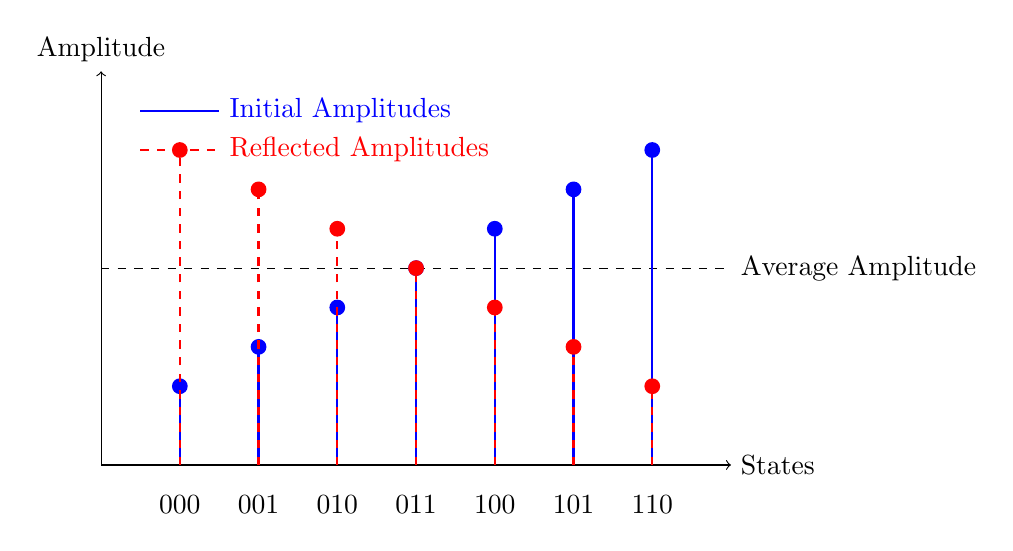
\begin{tikzpicture}
  % Draw axes
  \draw[->] (0,0) -- (8,0) node[right]{States};
  \draw[->] (0,0) -- (0,5) node[above]{Amplitude};

  % Draw average amplitude line
  \draw[dashed] (0,2.5) -- (8,2.5) node[right]{Average Amplitude};

  % Draw initial amplitudes
  \foreach \x/\y in {1/1, 2/1.5, 3/2, 4/2.5, 5/3, 6/3.5, 7/4} {
    \draw[blue, thick] (\x,0) -- (\x,\y);
    \fill[blue] (\x,\y) circle (0.1);
  }

  % Draw reflected amplitudes
  \foreach \x/\y in {1/4, 2/3.5, 3/3, 4/2.5, 5/2, 6/1.5, 7/1} {
    \draw[red, thick, dashed] (\x,0) -- (\x,\y);
    \fill[red] (\x,\y) circle (0.1);
  }

  % Labels
  \node at (1,-0.5) {\(\ket{000}\)};
  \node at (2,-0.5) {\(\ket{001}\)};
  \node at (3,-0.5) {\(\ket{010}\)};
  \node at (4,-0.5) {\(\ket{011}\)};
  \node at (5,-0.5) {\(\ket{100}\)};
  \node at (6,-0.5) {\(\ket{101}\)};
  \node at (7,-0.5) {\(\ket{110}\)};

  % Legend
  \draw[blue, thick] (0.5,4.5) -- (1.5,4.5) node[right]{Initial Amplitudes};
  \draw[red, thick, dashed] (0.5,4) -- (1.5,4) node[right]{Reflected Amplitudes};
\end{tikzpicture}
\end{center}

\vspace{0.3cm}

The blue bars represent the initial amplitudes of the states, and the red
dashed bars represent the amplitudes after inversion about the mean. The
marked state's amplitude is amplified, while the amplitudes of the other
states are reduced.


%%%%%%%%%%%%%%%%%%%%%%%%%%%%%%%%%%%%%%%%%%%%%%%%%%
% 2-Qubit Example
%%%%%%%%%%%%%%%%%%%%%%%%%%%%%%%%%%%%%%%%%%%%%%%%%%
\subsection*{2-Qubit Example}

To build intuition, consider the case \( n=2 \) (i.e., \( N=4 \)) with the winning
state chosen as \(\ket{11}\).

\vspace{0.3cm}

\textbf{Oracle:} For a 2-qubit system, the Oracle \(O\) can be implemented as a
controlled-\(Z\) (CZ) gate:
\[
  CZ =
  \begin{pmatrix}
    1 & 0 & 0 & 0 \\
    0 & 1 & 0 & 0 \\
    0 & 0 & 1 & 0 \\
    0 & 0 & 0 & -1
  \end{pmatrix},
\]

which multiplies the state \(\ket{11}\) by \(-1\).

\vspace{0.3cm}

\textbf{Diffusion Operator:} For 2 qubits, the diffusion operator is given by:

\[
  D = H^{\otimes 2}\; X^{\otimes 2}\; CZ\; X^{\otimes 2}\; H^{\otimes 2}.
\]

\vspace{0.3cm}

\textbf{2-Qubit Grover Circuit:}

\[
\begin{quantikz}
  \lstick{$\ket{0}$} & \gate{H} & \ctrl{1} & \gate{H} & \gate{X} & \qw & \ctrl{1} & \qw & \gate{X} & \gate{H} & \meter{} \\
  \lstick{$\ket{0}$} & \gate{H} & \ctrl{0} & \gate{H} & \gate{X} & \gate{H} & \gate{X} & \gate{H} & \gate{X} & \gate{H} & \meter{}
\end{quantikz}
\]

\vspace{0.3cm}

\noindent
\textbf{Explanation:}

\begin{itemize}
  \item \textbf{Oracle:} The Oracle adds a phase of \(-1\) to the winning
    state \(\ket{11}\), effectively marking it.
  \item \textbf{Diffusion Operator:} The diffusion circuit (implemented as
    \(H\;X\;CZ\;X\;H\)) reflects all amplitudes about the average. This
    inversion about the mean amplifies the amplitude of the marked state.
\end{itemize}

%%%%%%%%%%%%%%%%%%%%%%%%%%%%%%%%%%%%%%%%%%%%%%%%%%
% Algorithm Walkthrough and Pseudocode
%%%%%%%%%%%%%%%%%%%%%%%%%%%%%%%%%%%%%%%%%%%%%%%%%%

\index{Grover's Search Algorithm!pseudocode}
\subsection*{Walkthrough of the Algorithm and Generalization to \(n\) Qubits}

Grover's algorithm can be summarized in the following pseudocode:

\begin{algorithm}[H]
  \caption{Grover's Search Algorithm}
  \KwIn{A function \( f: \{0,1\}^n \rightarrow \{0,1\} \) with a unique
  marked state \( x_0 \) such that \( f(x_0) = 1 \).}
  \KwOut{The marked element \( x_0 \).}

  \textbf{Initialize:} Set the quantum state to \( \ket{\psi} \gets
  \ket{0}^{\otimes n} \).\\

  Apply \( H^{\otimes n} \) to obtain the uniform superposition:

  \[
    \ket{s} = H^{\otimes n}\ket{0}^{\otimes n} = \frac{1}{\sqrt{2^n}} \sum_{x
    \in \{0,1\}^n} \ket{x}.
  \]

  \For{\( i = 1 \) \KwTo \( \left\lfloor \frac{\pi}{4}\sqrt{2^n}
  \right\rfloor \)}{

    Apply the Oracle \( O \) which performs:

    \[
      O\ket{x} = (-1)^{f(x)}\ket{x},
    \]
    (i.e., flip the phase of the marked state).\;

    Apply the Diffusion Operator \( D = 2\ket{s}\bra{s} - I \)
    (which reflects amplitudes about the average).\;
  }

  Measure the state in the computational basis to obtain \( x_0 \).\;

\end{algorithm}

\vspace{0.3cm}

\noindent
\textbf{Detailed Explanation:}
\begin{enumerate}
  \item \textbf{Initialization:} All qubits are set to \(\ket{0}\) and then
    put into an equal superposition via \(H^{\otimes n}\).

  \item \textbf{Oracle Application:} The Oracle selectively flips the phase
    of the winning state(s) (e.g., for the marked state \(\ket{w}\),
    \(O\ket{w} = -\ket{w}\)).

  \item \textbf{Diffusion (Inversion about the Mean):} This operator reflects
    the state vector about the average amplitude. Geometrically, one can
    view the process as a rotation in a two-dimensional subspace.

  \item \textbf{Iteration:} Repeating the Oracle and Diffusion steps
    approximately \( \sqrt{2^n} \) times amplifies the probability amplitude of
    the marked state.

  \item \textbf{Measurement:} Finally, a measurement in the computational
    basis yields the marked element with high probability.
\end{enumerate}

This algorithm demonstrates how quantum algorithms can achieve a quadratic
speedup over classical brute-force search methods.

%%%%%%%%%%%%%%%%%%%%%%%%%%%%%%%%%%%%%%%%%%%%%%%%%%
% End of Lecture 9
%%%%%%%%%%%%%%%%%%%%%%%%%%%%%%%%%%%%%%%%%%%%%%%%%%

\section{Lecture 10: Quantum Logic Gates, Applying Grover's Search Algorithm
to SAT}\label{sec:lecture10}

%%%%%%%%%%%%%%

\subsection*{Review Question from Last Lecture}

\qs{Function of the Hadamard Layer in Grover's Algorithm}{
  Why does Grover's algorithm apply a Hadamard ($H$) gate to each of the $n$
  qubits at the beginning of the circuit?
}

\sol{
  The purpose of the Hadamard layer is that it allows up to work with all
  bitstring permutations simultaneously by putting all states in equal
  superposition.

  The Hadamard layer initializes the system in a uniform superposition of all
  possible $2^n$ states, allowing Grover's algorithm to explore all bitstring
  permutations simultaneously. For $n$ qubits starting at $|0\rangle^{\otimes
  n}$, applying $H^{\otimes n}$ yields:
  \[
    |s\rangle = H^{\otimes n} |0\rangle^{\otimes n} = \frac{1}{\sqrt{2^n}}
    \sum_{x \in \{0,1\}^n} |x\rangle.
  \]

  This equal superposition ensures that the algorithm can amplify the
  amplitude of the solution state(s) efficiently.
}

%%%%%%%%%%%%%

\subsection*{Quantum Implementations of Classical Logic Gates}

\index{quantum gates!OR gate}
\subsubsection*{OR Gate}

The quantum OR gate computes $c = a \lor b$ using a combination of CNOT and
Toffoli gates. Below is the two-way OR implementation:
\[
  \begin{quantikz}
    \lstick{$|a\rangle$} & \ctrl{1} & \ctrl{2} & \qw \\
    \lstick{$|b\rangle$} & \ctrl{1} & \targ{} & \qw \\
    \lstick{$|c\rangle$} & \targ{} & \targ{} & \qw
  \end{quantikz}
\]

\textbf{Truth Table:}
\[
  \begin{array}{ccc|c}
    a & b & c_{\text{in}} & c_{\text{out}} = a \lor b \\
    \hline
    0 & 0 & 0 & 0 \\
    0 & 1 & 0 & 1 \\
    1 & 0 & 0 & 1 \\
    1 & 1 & 0 & 1 \\
  \end{array}
\]

The circuit uses CCNOT (Toffoli) to set $c$ if both $a$ and $b$ are 1, then
CNOTs to flip $c$ if either $a$ or $b$ is 1, effectively computing OR. NOT
gates ($X$) can be added to inputs for negated terms (e.g., $\neg a \lor \neg
b$).

\index{quantum gates!NOR gate}
\subsubsection*{NOR Gate}

A NOR gate ($c = \neg (a \lor b)$) can be implemented by adding an $X$ gate
on the output qubit after the OR circuit:
\[
  \begin{quantikz}
    \lstick{$|a\rangle$} & \ctrl{1} & \ctrl{2} & \qw \\
    \lstick{$|b\rangle$} & \ctrl{1} & \targ{} & \qw \\
    \lstick{$|c\rangle$} & \targ{} & \targ{} & \gate{X} & \qw
  \end{quantikz}
\]


\textbf{Truth Table:}
\[
  \begin{array}{ccc|c}
    a & b & c_{\text{in}} & c_{\text{out}} = \neg (a \lor b) \\
    \hline
    0 & 0 & 0 & 1 \\
    0 & 1 & 0 & 0 \\
    1 & 0 & 0 & 0 \\
    1 & 1 & 0 & 0 \\
  \end{array}
\]

\index{quantum gates!AND gate}
\subsubsection*{AND Gate}

An AND gate ($c = a \land b$) is directly implemented with a Toffoli gate:
\[
  \begin{quantikz}
    \lstick{$| a \rangle$} & \ctrl{1} & \qw \\
    \lstick{$| b \rangle$} & \ctrl{1} & \qw \\
    \lstick{$| c \rangle$} & \targ{} & \qw
  \end{quantikz}
\]

\textbf{Truth Table:}
\[
  \begin{array}{ccc|c}
    a & b & c_{\text{in}} & c_{\text{out}} = a \land b \\
    \hline
    0 & 0 & 0 & 0 \\
    0 & 1 & 0 & 0 \\
    1 & 0 & 0 & 0 \\
    1 & 1 & 0 & 1 \\
  \end{array}
\]

\index{quantum gates!NAND gate}
\subsubsection*{NAND Gate}
A NAND gate ($c = \neg (a \land b)$) adds an $X$ gate after the AND:
\[
  \begin{quantikz}
    \lstick{$|a\rangle$} & \ctrl{1} & \qw \\
    \lstick{$|b\rangle$} & \ctrl{1} & \qw \\
    \lstick{$|c\rangle$} & \targ{} & \gate{X} & \qw
  \end{quantikz}
\]

\textbf{Truth Table:}
\[
  \begin{array}{ccc|c}
    a & b & c_{\text{in}} & c_{\text{out}} = \neg (a \land b) \\
    \hline
    0 & 0 & 0 & 1 \\
    0 & 1 & 0 & 1 \\
    1 & 0 & 0 & 1 \\
    1 & 1 & 0 & 0 \\
  \end{array}
\]

%%%%%%%%%%%%%

\subsection*{Applying Grover's Algorithm to SAT}

\index{quantum kickback}
\dfn{Quantum Kickback}{
  Quantum kickback occurs when a controlled operation transfers a phase from
  the target qubit to the control qubit(s). In Grover's algorithm, the oracle
  uses this to mark solution states. Consider a simple example with a
  controlled-$X$ and phase:
  \[
    \begin{quantikz}
      \lstick{$|+\rangle$} & \ctrl{1} & \qw \\
      \lstick{$|-\rangle$} & \targ{} & \qw
    \end{quantikz}
  \]

  Initial state: $|+\rangle|-\rangle = \frac{1}{\sqrt{2}}(|0\rangle +
  |1\rangle) \otimes \frac{1}{\sqrt{2}}(|0\rangle - |1\rangle) =
  \frac{1}{2}(|00\rangle - |01\rangle + |10\rangle - |11\rangle)$.

  After CNOT:
  \[
    \frac{1}{2}(|00\rangle - |01\rangle + |11\rangle - |10\rangle) =
    \frac{1}{\sqrt{2}}(|0\rangle - |1\rangle) \otimes \frac{1}{\sqrt{2}}(|0\rangle - |1\rangle) =
    |-\rangle|-\rangle.
  \]

  The phase of the target ($|-\rangle$) "kicks back" to the control, flipping
  its relative phase. In Grover's oracle, a multi-controlled $X$ on an
  ancilla in $|-\rangle$ state marks solutions with a $-1$ phase.
}

\paragraph{Implications of Quantum Kickback}\label{par:Implications of Quantum Kickback}

Quantum kickback enables efficient phase marking in Grover’s algorithm
without altering the computational basis states directly. It implies that:

\begin{itemize}
  \item Ancilla qubits in superposition (e.g., $|-\rangle$) can encode
    solution conditions.\footnote{\textbf{ancilla}: extra qubits (beyond the
    clauses) that we need to complete the complete the computation}

  \item The oracle’s design must ensure correct phase inversion for all
    satisfying assignments.

  \item When designing algorithms, we leverage kickback to avoid classical
    computation of each clause, reducing circuit depth and enhancing quantum
    speedup.
\end{itemize}

\index{Grover's Search Algorithm!Alexandria Ship Example@\textit{Alexandria
Ship Example}}
\ex{Alexandria Ship Example}{

  In 48 BCE Alexandria, a merchant must maximize passengers on a ship to
  Italy under these constraints:

  \begin{enumerate}
    \item \textit{Arsinoe (A)} won’t go if Cleopatra (C) is on the ship:
      $\neg A \lor \neg C$.

    \item \textit{Arsinoe} won’t go alone: $\neg A \lor J \lor P$.

    \item \textit{Ptolemy (P)} only goes if Julius Caesar (J) goes: $\neg P
      \lor J$.

    \item \textit{Ptolemy} won’t go if Cleopatra is on: $\neg P \lor \neg C$.

    \item \textit{Julius Caesar} must go: $J$.

    \item \textit{Cleopatra} won’t go if Julius Caesar is on: $\neg C \lor
      \neg J$.
  \end{enumerate}

  \textbf{Goal:} Find the maximum number of passengers (A, C, J, P)
  satisfying all constraints using Grover’s algorithm.
}

\paragraph{Creating SAT Clauses}\label{par:Creating SAT Clauses} % (fold)

The problem is a SAT instance with clauses:

\begin{enumerate}
  \item $\neg A \lor \neg C$ (Arsinoe-Cleopatra conflict).
  \item $\neg A \lor J \lor P$ (Arsinoe not alone).
  \item $\neg P \lor J$ (Ptolemy needs Caesar).
  \item $\neg P \lor \neg C$ (Ptolemy-Cleopatra conflict).
  \item $J$ (Caesar must go).
  \item $\neg C \lor \neg J$ (Cleopatra-Caesar conflict).
\end{enumerate}

These are implemented as OR gates in the quantum circuit, with an
ancilla qubit per clause. The final ancilla ($q_9$) computes the AND of all
clauses using a multi-controlled $X$, marking satisfying assignments with a
phase flip.

% paragraph Creating SAT Clauses (end)

\subsubsection*{\texttt{Cirq} Implementation}

Below is the Cirq code with detailed explanations:

\begin{minted}[linenos,highlightlines={6-10},highlightcolor=yellow!20]{python}
import cirq

# Qubits: A=0, C=1, J=2, P=3, clause ancillas=4-8, final output=9
qubits = cirq.LineQubit.range(10)

def twoway_OR(circuit, a, b, c, not_a, not_b):
    if not_a: circuit.append(cirq.X(a))
    if not_b: circuit.append(cirq.X(b))
    circuit.append(cirq.CCNOT(a, b, c))  # AND to target
    circuit.append(cirq.CNOT(a, c))      # OR logic
    circuit.append(cirq.CNOT(b, c))
    if not_a: circuit.append(cirq.X(a))
    if not_b: circuit.append(cirq.X(b))
    return circuit
\end{minted}
\textit{Lines 6-10}: Implements $c = a \lor b$ by computing AND then adding
single-qubit terms, with optional inversions for negated inputs.

\begin{minted}[linenos,highlightlines={11-14}]{python}
clauses_circuit = cirq.Circuit()
twoway_OR(clauses_circuit, qubits[0], qubits[1], qubits[4], 1, 1)  # A or not C
threeway_OR(clauses_circuit, qubits[0], qubits[2], qubits[3], qubits[5], 1, 0, 0)  # not A or J or P
twoway_OR(clauses_circuit, qubits[1], qubits[2], qubits[6], 1, 1)  # not C or not J
twoway_OR(clauses_circuit, qubits[1], qubits[3], qubits[7], 1, 1)  # not C or not P
twoway_OR(clauses_circuit, qubits[2], qubits[3], qubits[8], 0, 1)  # J or not P

oracle_circuit = cirq.Circuit()
oracle_circuit.append(clauses_circuit)
oracle_circuit.append(cirq.X(qubits[9]).controlled_by(qubits[2], qubits[4], qubits[5],
                                                      qubits[6], qubits[7], qubits[8]))
oracle_circuit.append(clauses_circuit)
\end{minted}
\textit{Lines 11-14}: The oracle computes all clauses, then uses a
multi-controlled $X$ on $q_9$ (in $|-\rangle$ state) to flip the phase of
satisfying states, leveraging kickback.

\begin{minted}[linenos,highlightlines={5-7}]{python}
final_circuit = cirq.Circuit()
final_circuit.append(cirq.H.on_each(qubits[0:4]))  # Superposition
final_circuit.append(cirq.X(qubits[9]))            # Prepare ancilla
final_circuit.append(cirq.H(qubits[9]))
final_circuit.append(oracle_circuit)
final_circuit.append(diffusion_circuit)            # From notebook
final_circuit.append(cirq.measure(qubits[0:4][::-1], key='PJCA'))
\end{minted}

\textit{Lines 5-7}: Initializes input qubits in superposition and ancilla in
$|-\rangle$, applies oracle and diffusion, then measures.

\paragraph{Results from the Circuit}\label{par:Results from the Circuit}
Running the circuit with 8192 repetitions yields:

\begin{verbatim}
Counter({5: 2079, 13: 2043, 12: 2037, 4: 2033})
\end{verbatim}

\noindent
Converting to binary (PJCA order):

\begin{itemize}
  \item $5 = 0101$: $P=0, J=1, C=0, A=1$ (J, A).
  \item $13 = 1101$: $P=1, J=1, C=0, A=1$ (P, J, A).
  \item $12 = 1100$: $P=1, J=1, C=0, A=0$ (P, J).
  \item $4 = 0100$: $P=0, J=1, C=0, A=0$ (J).
\end{itemize}

All solutions have $J=1$ (Caesar goes), $C=0$ (Cleopatra stays), and vary in
A and P, satisfying all constraints. The maximum passengers (3) is $P=1, J=1,
A=1$, excluding Cleopatra, optimizing the merchant’s goal.

We have shown how Grover’s Search Algorithm efficiently solves this SAT
problem, amplifying valid configurations quadratically faster than classical
search!

\emph{However}, when we look at the representation of this circuit, it is
clear that there are some optimizations that we can do to make it have a much
shallower depth and not rely on so many ancilla qubits--- which we will fix
in the next chapter.

%%%%%%%%%%%%%%%%%%%%%%%%%%%%%%%%%%%%%%%%%%%%%%
% End of Lecture 10
%%%%%%%%%%%%%%%%%%%%%%%%%%%%%%%%%%%%%%%%%%%%%%

\section{Lecture 11: Quantum Circuit Optimizations}\label{sec:lecture11}

The biggest sources of inefficiencies from the Grover's Search circuit that
we saw at the end of the last lecture were:

\begin{enumerate}
  \item The way in which we implemented the multi-way OR gates.

  \item The extensive use of ancilla qubits.
\end{enumerate}

We will address both of these inefficiencies to get a shallower and simpler
circuit.

\subsection*{More Efficient OR Gate Implementation}

% fill me in

\subsection*{Reducing Ancilla Qubits}

\subsubsection*{Converting from CNF to ANF}

In the last lecture, we wrote the clauses for the Alexandria ship problem using
conjunctive normal form (exclusively using OR and NOT for each clause). However,
by converting to using algebraic normal form (exclusively using AND and XOR), we
will only have to use $O(1)$ additional ancilla for this problem\footnote{It is
guaranteed that this conversion from CNF to ANF will produce similar results for
all problems.}, as opposed to the original $O(\text{# of clauses})$ addition
ancilla from the original CNF implementation.

% fill me in with implementation details and all that jazz



% ==============================
% PHASE III: ADVANCED
% ==============================
\chapter{Phase III: Advanced Quantum Algorithms}

% ● Introduction to variational quantum algorithms
% ● Training and optimization of variational algorithms
\section{Lecture 12: Introduction to Variational Quantum
Algorithms}\label{sec:lecture12}

Before we can begin discussions on Quantum Approximate Optimization
Algorithms (QAOA)\footnote{This class of algorithms are also interchangeably
  referred to as "Quantum Alternating Operator Ansatz," with "ansatz" meaning
"guess" in German for reasons that will become clear in the next lectures.},
we must first refine our conception of the classes of algorithms that are
affected by quantum computing. Additionally, we will get an introduction to a
broader class of algorithms called \emph{variational quantum algorithms
(VQA)}, of which QAOA is a subset.

\subsection*{Classes of Algorithms}

We can group algorithms into two classes: (1) those with proven quantum
speedup and (2) those with not fully proven quantum speedup.

\index{proven quantum speedup algorithms}
\subsubsection*{Proven Quantum Speedup Algorithms}

We have already seen one of these algorithms with Grover's Algorithm, which
has proven quadratic speedup. This means that for a search problem over $N$
items, Grover’s algorithm reduces the complexity from $O(N)$ in classical
computing to $O(\sqrt{N})$ in the quantum domain. Other examples include:

\begin{itemize}
  \index{proven quantum speedup algorithms!Shor's Algorithm}
  \item \textbf{Shor’s Algorithm}: Provides exponential speedup for integer
    factorization, reducing the complexity from $O(\exp((\log N)^{1/3}))$ to
    $O((\log N)^3)$.

    \index{proven quantum speedup algorithms!QFT}
  \item \textbf{Quantum Fourier Transform (QFT)}: Used in phase estimation,
    offering exponential speedup over classical FFT for certain applications.
\end{itemize}

These algorithms leverage quantum superposition, entanglement, and
interference to achieve rigorously proven advantages, often validated through
mathematical analysis of their unitary operators and measurement probabilities.

\index{heuristic quantum algorithms}
\subsubsection*{Heuristic Quantum Algorithms}

Heuristic quantum algorithms lack a fully proven speedup but show promise
based on empirical evidence or specific problem instances. These include:

\begin{itemize}
  \index{heuristic quantum algorithms!QAOA}
  \item \textbf{Quantum Approximate Optimization Algorithm (QAOA)}: A hybrid
    quantum-classical approach for combinatorial optimization, conjectured to
    offer speedup for certain graphs, though the exact advantage remains
    under investigation.

    \index{heuristic quantum algorithms!quantum machine learning}
  \item \textbf{Quantum Machine Learning (QML)}: Algorithms like quantum
    support vector machines or clustering may provide polynomial or
    context-specific speedups, often relying on variational techniques (see
    below).

    \index{heuristic quantum algorithms!quantum stimulation}
  \item \textbf{Quantum Simulation}: Simulating quantum systems (e.g.,
    molecular dynamics) is believed to be exponentially faster than classical
    methods, but the speedup depends on the Hamiltonian and is not
    universally proven.
\end{itemize}

These algorithms often use an "ansatz"—a parameterized guess for the quantum
state—adjusted iteratively, making their performance problem-dependent and
harder to analyze theoretically.

%%%%%%%%%%%

\index{Variational Quantum Algorithms}
\subsection*{Variational Quantum Algorithms (VQA)}

Variational Quantum Algorithms (VQA) are a class of hybrid quantum-classical
algorithms that optimize a cost function by varying circuit parameters to
achieve an objective. As noted in the lecture notes, they involve "varying
circuit parameters," typically through a parameterized quantum circuit (the
ansatz), followed by classical optimization of the parameters based on
measurement outcomes. Key features include:

\begin{itemize}
  \item \textbf{Hybrid Nature}: A quantum circuit prepares a state
    $\ket{\psi(\theta)}$ with parameters $\theta$, measured to compute a cost
    $C(\theta)$, which a classical optimizer (e.g., gradient descent) minimizes.

  \item \textbf{Applications}: VQAs are used for optimization (e.g., QAOA),
    quantum chemistry (e.g., Variational Quantum Eigensolver, VQE), and
    machine learning.

  \item \textbf{Flexibility}: The ansatz can be tailored to the problem,
    balancing expressiveness with hardware constraints like qubit count and
    gate depth.
\end{itemize}

The general process is depicted as:

\[
  \ket{\psi(\theta)} \xrightarrow{\text{varying circuit}} \text{Measure }
  C(\theta) \xrightarrow{\text{classical optimization}} \theta_{\text{opt}}
\]

\textbf{Advantages:}
\begin{itemize}
  \item Robust to noise in near-term quantum devices (NISQ).

  \item Scales with available quantum resources, unlike exact algorithms
    requiring deep circuits.
\end{itemize}

\textbf{Challenges:}
\begin{itemize}
  \item Barren plateaus in the optimization landscape can hinder convergence.

  \item Ansatz design impacts solution quality and computational cost.

\end{itemize}

\ex{Toy Example: Bell State Preparation}{
  A simple VQA example is preparing a Bell state, such as $\ket{\Phi^+} =
  \frac{\ket{00} + \ket{11}}{\sqrt{2}}$, using a parameterized circuit.
  Consider a circuit with a rotation gate $R_y(\theta)$ on one qubit followed
  by a CNOT:

  \textbf{Circuit Diagram:}
  \[
    \begin{quantikz}
      \lstick{$\ket{0}$} & \gate{R_y(\theta)} & \ctrl{1} & \qw \\
      \lstick{$\ket{0}$} & \qw & \targ{} & \qw
    \end{quantikz}
  \]

  \textbf{Objective}: Minimize the cost function $C(\theta) = 1 - |\langle
  \Phi^+ | \psi(\theta) \rangle|^2$, where $\ket{\psi(\theta)} = \text{CNOT}
  \cdot (R_y(\theta) \ket{0}) \otimes \ket{0}$. For $\theta = \pi/2$,
  $R_y(\pi/2)\ket{0} = \frac{\ket{0} + \ket{1}}{\sqrt{2}}$, and the circuit
  yields the Bell state exactly.

  \textbf{Truth Table (post-measurement probabilities):}
  \[
    \begin{array}{cc|c}
      q_0 & q_1 & P(q_0, q_1) \\
      \hline
      0 & 0 & 0.5 \\
      0 & 1 & 0 \\
      1 & 0 & 0 \\
      1 & 1 & 0.5 \\
    \end{array}
  \]

  This toy example illustrates parameter tuning to achieve a target state, a
  core concept in VQAs.
}

%%%%%%%%% Cirq code

Below is a Cirq implementation of the Bell state preparation, adapted from
the homework’s quantum circuit style:

\begin{minted}[linenos]{python}
import cirq
import numpy as np

# Define qubits
q0, q1 = cirq.LineQubit.range(2)

# Parameterized circuit
theta = np.pi / 2  # Optimal parameter
circuit = cirq.Circuit(
    cirq.ry(theta).on(q0),  # Rotation
    cirq.CNOT(q0, q1)       # Entanglement
)

# Simulate
simulator = cirq.Simulator()
result = simulator.simulate(circuit)
state = result.final_state_vector
print("Final state:", np.round(state, 3))

# Measure (8192 shots)
circuit.append(cirq.measure(q0, q1, key='result'))
samples = simulator.run(circuit, repetitions=8192)
counts = samples.histogram(key='result')
print("Counts:", counts)
\end{minted}

\textbf{Output Explanation:}
\begin{itemize}
  \item \textit{State Vector}: Approximately $[0.707, 0, 0, 0.707]$, matching
    $\ket{\Phi^+}$.

  \item \textit{Counts}: Roughly $\{0: 4096, 3: 4096\}$ (binary 00 and 11),
    confirming 50\% probability each.
\end{itemize}

This demonstrates a VQA’s ability to prepare a desired quantum state via
parameter optimization, foundational to more complex algorithms like QAOA.

%%%%%%%%%%%%%%%%%%%%%%%%%%%%%%%%%%%%%%%%%%%%%%
% End of Lecture 12
%%%%%%%%%%%%%%%%%%%%%%%%%%%%%%%%%%%%%%%%%%%%%%


% ● Introduction to quantum optimization problems
% ● Quantum approximate optimization algorithm (QAOA)
\section{Lecture 13: Introduction to Quantum Approximate Optimization
Algorithms}\label{sec:lecture13}

\subsubsection*{Review}

\qs{VQA}{
  What varies when running a variational quantum algorithm?
}

\sol{
  Rotation gate angles.
}

\qs{Ansatz in QAOA}{
  What does "ansatz" refer to in Quantum Alternating Operator Ansatz (aka QAOA)?
}

\sol{
  Making a guess about the quantum circuit to use for optimization. In QAOA,
  the ansatz is a parameterized circuit alternating between cost and mixing
  Hamiltonians, designed to approximate the optimal state for a problem, with
  parameters tuned iteratively.
}


%%%%%%%%%%%%%%%%%

\index{Quantum Approximate Optimization Algorithms}
\subsubsection*{Quantum Approximate Optimization Algorithms}

The Quantum Approximate Optimization Algorithm (QAOA) is a hybrid
quantum-classical algorithm within the VQA family, tailored for combinatorial
optimization problems (e.g., \textsc{Max-Cut}, graph coloring). Introduced by
Farhi et al.\footnote{"A Quantum Approximate Optimization Algorithm":
https://arxiv.org/abs/1411.4028}, it approximates the ground state of a cost
Hamiltonian by alternating two types of unitary operators, controlled by
parameters optimized classically.

\vspace{0.3cm}

\noindent
\textbf{Core Idea:}
\begin{itemize}
  \index{Quantum Approximate Optimization Algorithms!Cost Hamiltonian}
  \item \textbf{Cost Hamiltonian ($H_C$)}: Encodes the problem’s objective,
    e.g., $H_C = \sum_{\langle i,j \rangle} Z_i Z_j$ for Max-Cut, where lower
    energy states correspond to better solutions.

  \item \textbf{Mixing Hamiltonian ($H_M$)}: Typically $H_M = \sum_i X_i$,
    drives exploration across the solution space.

  \index{Quantum Approximate Optimization Algorithms!ansatz}
  \item \textbf{Ansatz State}: $\ket{\psi(\gamma, \beta)} = \prod_{p=1}^P
    e^{-i\beta_p H_M} e^{-i\gamma_p H_C} \ket{s}$, where $\ket{s}$ is a
    uniform superposition (e.g., $H^{\otimes n} \ket{0}^{\otimes n}$), and
    $P$ is the number of layers.

  \item \textbf{Goal}: Find $\gamma = (\gamma_1, \ldots, \gamma_P)$ and
    $\beta = (\beta_1, \ldots, \beta_P)$ minimizing $\langle \psi(\gamma,
    \beta) | H_C | \psi(\gamma, \beta) \rangle$.

\end{itemize}

\vspace{0.3cm}

\noindent
\textbf{Algorithm Steps:}
\begin{enumerate}
  \item \textbf{Initialize}: For $n$ qubits, apply Hadamard gates: $\ket{s} =
    H^{\otimes n} \ket{0}^{\otimes n} = \frac{1}{\sqrt{2^n}} \sum_{x \in
    \{0,1\}^n} \ket{x}$. (Your note `$10 \mathrm{~N} \rightarrow \mathrm{H}$`
    suggests $n=10$.)

  \item \textbf{Apply Ansatz}: For $p=1$ to $P$, apply $e^{-i\gamma_p H_C}$
    (cost evolution) and $e^{-i\beta_p H_M}$ (mixing evolution).

  \item \textbf{Measure}: Compute $\langle H_C \rangle$ by measuring in the
    computational basis.

  \item \textbf{Optimize}: Use a classical algorithm (e.g., gradient descent)
    to adjust $\gamma_p$ and $\beta_p$.

  \item \textbf{Repeat}: Iterate until $\langle H_C \rangle$ converges to an
    approximate minimum.

\end{enumerate}

\subsubsection*{\textsc{Max-Cut} Example}

Consider a 4-node cycle graph with edges $\{(0,1), (1,2), (2,3), (3,0)\}$,
weights $w_{ij} = 1$. The Max-Cut problem seeks a partition maximizing cut
edges.

\vspace{0.3cm}

\noindent
\textbf{Cost Hamiltonian:}
\[
  H_C = Z_0 Z_1 + Z_1 Z_2 + Z_2 Z_3 + Z_3 Z_0
\]

Eigenstate $\ket{0101}$ (alternating partition) has eigenvalue $-4$ (4 cuts,
optimal).

\textbf{Mixing Hamiltonian:}
\[
  H_M = X_0 + X_1 + X_2 + X_3
\]

\textbf{Ansatz Circuit ($P=1$):}

\[
  \begin{quantikz}
    \lstick{$q_0: \ket{0}$} & \gate{H} & \gate{e^{-i\gamma Z_0 Z_1}} & \gate{e^{-i\gamma Z_3 Z_0}} & \gate{R_X(2\beta)} & \meter{} \\
    \lstick{$q_1: \ket{0}$} & \gate{H} & \gate[2]{Z_1 Z_2} & \qw & \gate{R_X(2\beta)} & \meter{} \\
    \lstick{$q_2: \ket{0}$} & \gate{H} & \qw & \gate[2]{Z_2 Z_3} & \gate{R_X(2\beta)} & \meter{} \\
    \lstick{$q_3: \ket{0}$} & \gate{H} & \qw & \qw & \gate{R_X(2\beta)} & \meter{}
  \end{quantikz}
\]

\begin{itemize}

  \item $e^{-i\gamma Z_i Z_j}$: Use CNOTs and $R_Z(2\gamma)$, since
    $e^{-i\theta Z_i Z_j} = \text{CNOT} \cdot (I \otimes R_Z(\theta)) \cdot
    \text{CNOT}$.

  \item $e^{-i\beta X_i}$: Direct $R_X(2\beta)$ gate.

\end{itemize}

\subsubsection*{Cirq Implementation}

Here’s a QAOA circuit for the 4-qubit Max-Cut with $P=1$:

\begin{minted}[linenos]{python}
import cirq
import numpy as np

# Qubits
qubits = cirq.LineQubit.range(4)

# Parameters (example)
gamma, beta = 0.5, 0.3

# Circuit
circuit = cirq.Circuit()
circuit.append(cirq.H.on_each(qubits))  # Superposition
# Cost terms
for i in range(4):
    circuit.append(cirq.ZZPowGate(exponent=2 * gamma/ np.pi).on(qubits[i], qubits[(i + 1) % 4]))
# Mixing terms
circuit.append(cirq.rx(2*beta).on_each(qubits))
# Measure
circuit.append(cirq.measure(*qubits, key='result'))

# Simulate
simulator = cirq.Simulator()
result = simulator.run(circuit, repetitions=8192)
counts = result.histogram(key='result')
print("Counts:", counts)
\end{minted}

\subsubsection*{Properties}

\textbf{Advantages:}
\begin{itemize}
  \item Works on NISQ devices with shallow circuits ($P$ small).
  \item $P \to \infty$ theoretically yields the exact solution (adiabatic limit).
\end{itemize}

\textbf{Limitations:}
\begin{itemize}
  \item Barren plateaus may trap optimization.
  \item Speedup not guaranteed; depends on problem and $P$.
\end{itemize}

\ex{Toy Example: 3-Qubit Triangle}{
  Graph: edges $(0,1), (1,2), (2,0)$, $H_C = Z_0 Z_1 + Z_1 Z_2 + Z_2 Z_0$.
  Max cut is 2 (e.g., $\ket{010}$). For $P=1$, QAOA with tuned $\gamma,
  \beta$ boosts $\ket{010}$ and $\ket{101}$ probabilities.
}

%%%%%%%%%%%%%%%%%%%%%%%%%%%%%%%%%%%%%%%%%%%%%%
% End of Lecture 13
%%%%%%%%%%%%%%%%%%%%%%%%%%%%%%%%%%%%%%%%%%%%%%

\section{Lecture 14: More on QAOA: Cost and Mixer Hamiltonians, Full
Circuit}\label{sec:lecture14}

\subsubsection*{Review}

\qs{QAOA Components}{
  What are the two main components that alternate in a QAOA circuit?
}

\sol{
  The two main components are:
  \begin{enumerate}
    \item \textbf{Cost evolution operator}: $e^{-i\gamma_p H_C}$, which
      encodes the problem's objective function

    \item \textbf{Mixing evolution operator}: $e^{-i\beta_p H_M}$, which
      explores the solution space
  \end{enumerate}
}

%%%%%%%%%%%%

\vspace{0.3cm}

\index{Quantum Approximate Optimization Algorithms!Cost Hamiltonians}
\subsubsection*{Cost Hamiltonians in Detail}

\dfn{Cost Hamiltonian}{The \textbf{Cost Hamiltonian} $H_C$ in QAOA encodes
  the objective function of the optimization problem. It is designed such that
  its ground state (lowest energy eigenstate) corresponds to the optimal
solution of the classical problem.}

\vspace{0.3cm}

\noindent
\textbf{Properties of Cost Hamiltonians:}
\begin{itemize}
  \item \textbf{Diagonal in computational basis}: $H_C$ is typically diagonal
    in the $Z$-basis, making measurements straightforward.

  \item \textbf{Problem-specific}: Each optimization problem requires a
    different $H_C$.

  \item \textbf{Locality}: Many practical $H_C$ terms involve only a few
    qubits (e.g., 2-local terms like $Z_i Z_j$ for \textsc{Max-Cut}).
\end{itemize}


\noindent
\ex{Max-$k$-SAT Cost Hamiltonian}{
  For the Max-$k$-SAT problem, each clause $c$ is encoded as an operator
  $C_c$. For example, the clause $(x_1 \lor \lnot x_2 \lor x_3)$ is encoded as:
  \[
    C_c = \frac{I - Z_1}{2} \cdot \frac{I + Z_2}{2} \cdot \frac{I - Z_3}{2}
  \]

  The overall cost Hamiltonian is:
  \[
    H_C = \sum_{c} \frac{1-C_c}{2}
  \]

  This gives higher energy to states that satisfy more clauses.
}

\begin{figure}[H]
  \centering
  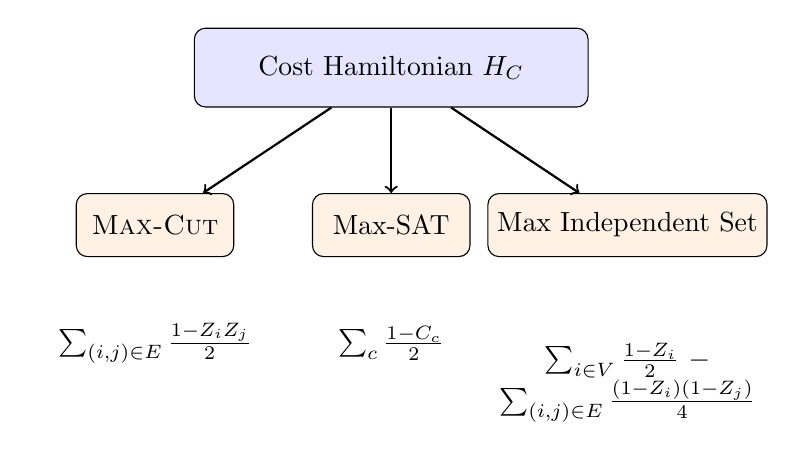
\begin{tikzpicture}
    \node[draw, rounded corners, fill=blue!10, minimum width=5cm, minimum height=1cm] (cost) at (0,0) {Cost Hamiltonian $H_C$};

    \node[draw, rounded corners, fill=orange!10, minimum width=2cm, minimum height=0.8cm] (maxcut) at (-3,-2) {\textsc{Max-Cut}};
    \node[draw, rounded corners, fill=orange!10, minimum width=2cm, minimum height=0.8cm] (maxsat) at (0,-2) {Max-SAT};
    \node[draw, rounded corners, fill=orange!10, minimum width=3.5cm, minimum height=0.8cm] (mis) at (3,-2) {Max Independent Set};

    \draw[->, thick] (cost) -- (maxcut);
    \draw[->, thick] (cost) -- (maxsat);
    \draw[->, thick] (cost) -- (mis);

    \node[align=center, text width=3cm] at (-3,-3.5) {$\sum_{(i,j) \in E} \frac{1-Z_i Z_j}{2}$};
    \node[align=center, text width=3cm] at (0,-3.5) {$\sum_{c} \frac{1-C_c}{2}$};
    \node[align=center, text width=3.5cm] at (3,-4) {$\sum_{i \in V} \frac{1-Z_i}{2} - \sum_{(i,j) \in E} \frac{(1-Z_i)(1-Z_j)}{4}$};
  \end{tikzpicture}
  \caption{Different cost Hamiltonians for various optimization problems}
  \label{fig:cost-hamiltonians}
\end{figure}

\vspace{0.3cm}

\index{Quantum Approximate Optimization Algorithms!Implementing Cost Hamiltonians}
\subsubsection*{Implementing Cost Hamiltonians}

The operator $e^{-i\gamma H_C}$ can be challenging to implement directly.
When $H_C$ consists of terms that commute with each other, we can decompose
the exponential:

\[
  e^{-i\gamma H_C} = e^{-i\gamma \sum_j h_j} = \prod_j e^{-i\gamma h_j}
\]

For the \textsc{Max-Cut} problem, each term is of the form $Z_i Z_j$, and we
can implement $e^{-i\gamma Z_i Z_j}$ using the following circuit:

\begin{figure}[H]
  \centering
  \begin{quantikz}
    \lstick{$q_i$} & \ctrl{1} & \qw & \ctrl{1} & \qw \\
    \lstick{$q_j$} & \targ{} & \gate{R_Z(2\gamma)} & \targ{} & \qw
  \end{quantikz}
  \caption{Circuit for implementing $e^{-i\gamma Z_i Z_j}$}
  \label{fig:zz-gate-implementation}
\end{figure}

\nt{
  The decomposition $e^{-i\gamma H_C} = \prod_j e^{-i\gamma h_j}$ is only
  valid when all terms $h_j$ commute. For non-commuting terms, more
  sophisticated techniques like Trotter-Suzuki decomposition are required.
}

\vspace{0.3cm}

\index{Quantum Approximate Optimization Algorithms!Mixer Hamiltonians}
\subsubsection*{Mixer Hamiltonians in Detail}

\dfn{Mixer Hamiltonian}{The \textbf{Mixer Hamiltonian} $H_M$ in QAOA drives
  the exploration of the solution space. It is typically chosen to be
  non-commuting with the cost Hamiltonian $H_C$ to enable transitions between
different states in the computational basis.}

\vspace{0.3cm}

\noindent
\textbf{Standard Mixer:}
\begin{itemize}
  \item The most common mixer is the transverse field: $H_M = \sum_{i=1}^n X_i$
  \item Implemented directly as $R_X(2\beta)$ gates on each qubit
  \item Allows exploration of the entire $2^n$ solution space
\end{itemize}

\begin{figure}[H]
  \centering
  \begin{quantikz}
    \lstick{$q_1$} & \gate{R_X(2\beta)} & \qw \\
    \lstick{$q_2$} & \gate{R_X(2\beta)} & \qw \\
    \lstick{$\vdots$} & \vdots & \vdots \\
    \lstick{$q_n$} & \gate{R_X(2\beta)} & \qw
  \end{quantikz}
  \caption{Circuit for implementing the standard mixer $e^{-i\beta \sum_i X_i}$}
  \label{fig:standard-mixer}
\end{figure}

\vspace{0.3cm}

\noindent
\textbf{Advanced Mixers:}
\begin{itemize}
  \item \textbf{Problem-specific mixers}: Designed to preserve constraints of
    the problem

  \item \textbf{XY mixers}: $H_M = \sum_{(i,j) \in E} (X_i X_j + Y_i Y_j)$
    for problems with hard constraints

  \item \textbf{Controlled mixers}: Conditionally apply mixing operations
    based on constraint satisfaction

\end{itemize}

\ex{XY Mixer for Number-Preserving Problems}{
  For problems where the total number of 1s must remain constant (e.g., graph
  coloring with a fixed number of colors), an XY mixer can be used:
  \begin{align}
    H_M^{XY} = \sum_{i < j} (X_i X_j + Y_i Y_j) = \sum_{i < j} (|01\rangle\langle10| + |10\rangle\langle01|)
  \end{align}

  This mixer only swaps 0s and 1s between qubits, preserving the total
  Hamming weight of the state. Implementation requires more complex gate
  sequences.

  \begin{figure}[H]
    \centering
    \begin{quantikz}
      \lstick{$q_i$} & \gate{H} & \ctrl{1} & \qw & \ctrl{1} & \gate{H} & \qw \\
      \lstick{$q_j$} & \gate{H} & \targ{} & \gate{R_Z(2\beta)} & \targ{} & \gate{H} & \qw
    \end{quantikz}
    \caption{Implementation of one term in the XY mixer}
    \label{fig:xy-mixer}
  \end{figure}
}

\vspace{0.3cm}

\index{Quantum Approximate Optimization Algorithms!Full QAOA Circuit}
\subsubsection*{Full QAOA Circuit Implementation}

\dfn{QAOA Circuit Depth}{The \textbf{QAOA circuit depth parameter} $P$
  determines how many alternating layers of cost and mixer operators are
  applied. Higher $P$ typically leads to better approximation quality but
increases circuit complexity.}

\vspace{0.3cm}

\noindent
\textbf{Circuit for QAOA with Depth $P$:}

\begin{figure}[H]
  \centering
  \begin{quantikz}
    \lstick{$q_1$} & \gate{H} & \gate[3]{e^{-i\gamma_1 H_C}} & \gate{R_X(2\beta_1)} & \gate[3]{e^{-i\gamma_2 H_C}} & \gate{R_X(2\beta_2)} & \ldots & \gate[3]{e^{-i\gamma_P H_C}} & \gate{R_X(2\beta_P)} & \meter{} \\
    \lstick{$q_2$} & \gate{H} & \qw & \gate{R_X(2\beta_1)} & \qw & \gate{R_X(2\beta_2)} & \ldots & \qw & \gate{R_X(2\beta_P)} & \meter{} \\
    \lstick{$q_n$} & \gate{H} & \qw & \gate{R_X(2\beta_1)} & \qw & \gate{R_X(2\beta_2)} & \ldots & \qw & \gate{R_X(2\beta_P)} & \meter{} \\
  \end{quantikz}
  \caption{General structure of a QAOA circuit with depth $P$}
  \label{fig:qaoa-general-circuit}
\end{figure}

\noindent
The circuit consists of:
\begin{enumerate}
  \item Initial state preparation: $H^{\otimes n}|0\rangle^{\otimes n}$

  \item $P$ repetitions of:
    \begin{itemize}
      \item Cost operator: $e^{-i\gamma_p H_C}$

      \item Mixer operator: $e^{-i\beta_p H_M}$
    \end{itemize}
  \item Final measurement in the computational basis

\end{enumerate}

\vspace{0.3cm}

\ex{Full \textsc{Max-Cut} QAOA Circuit for $P=2$}{
  For a 4-node cycle graph (\textsc{Max-Cut} problem) with $P=2$:

  \begin{figure}[H]
    \centering
    \begin{quantikz}
      \lstick{$q_0$} & \gate{H} & \gate{e^{-i\gamma_1 Z_0 Z_1}} & \gate{e^{-i\gamma_1 Z_0 Z_3}} & \gate{R_X(2\beta_1)} & \gate{e^{-i\gamma_2 Z_0 Z_1}} & \gate{e^{-i\gamma_2 Z_0 Z_3}} & \gate{R_X(2\beta_2)} & \meter{} \\
      \lstick{$q_1$} & \gate{H} & \qw & \gate{e^{-i\gamma_1 Z_1 Z_2}} & \gate{R_X(2\beta_1)} & \qw & \gate{e^{-i\gamma_2 Z_1 Z_2}} & \gate{R_X(2\beta_2)} & \meter{} \\
      \lstick{$q_2$} & \gate{H} & \qw & \qw & \gate{R_X(2\beta_1)} & \qw & \qw & \gate{R_X(2\beta_2)} & \meter{} \\
      \lstick{$q_3$} & \gate{H} & \qw & \gate{e^{-i\gamma_1 Z_2 Z_3}} & \gate{R_X(2\beta_1)} & \qw & \gate{e^{-i\gamma_2 Z_2 Z_3}} & \gate{R_X(2\beta_2)} & \meter{} \\
    \end{quantikz}
    \caption{QAOA circuit for \textsc{Max-Cut} on a 4-node cycle with $P=2$}
    \label{fig:maxcut-p2-circuit}
  \end{figure}

  Note that for clarity, the implementation of $e^{-i\gamma Z_i Z_j}$ with
  CNOT and $R_Z$ gates is not shown explicitly in this diagram.
}

\vspace{0.3cm}

\index{Quantum Approximate Optimization Algorithms!Parameter Optimization}
\subsubsection*{Parameter Optimization Strategies}

\dfn{QAOA Parameter Optimization}{The process of finding optimal values for
  the parameters $\gamma = (\gamma_1, \ldots, \gamma_P)$ and $\beta = (\beta_1,
  \ldots, \beta_P)$ to minimize the expectation value $\langle\psi(\gamma,
\beta)|H_C|\psi(\gamma, \beta)\rangle$.}

\vspace{0.3cm}

\noindent
\textbf{Classical Optimization Methods:}
\begin{itemize}
  \item \textbf{Gradient-free methods}: Nelder-Mead, COBYLA, Powell
  \item \textbf{Gradient-based methods}: BFGS, L-BFGS, SPSA
  \item \textbf{Global optimization}: Basin-hopping, Differential Evolution
\end{itemize}

\begin{algorithm}
  \caption{QAOA Parameter Optimization}
  \label{alg:parameter-optimization}
  \SetKwInOut{Input}{Input}
  \SetKwInOut{Output}{Output}

  \Input{Problem Hamiltonian $H_C$, Mixing Hamiltonian $H_M$, Number of layers $P$}
  \Output{Optimized parameters $\gamma^*$, $\beta^*$}

  Initialize parameters $\gamma = (\gamma_1, \ldots, \gamma_P)$ and $\beta = (\beta_1, \ldots, \beta_P)$\;
  Initialize optimizer (e.g., COBYLA, BFGS)\;

  \SetKwFunction{CostFunction}{CostFunction}
  \SetKwProg{Fn}{Function}{:}{}
  \Fn{\CostFunction{$\gamma, \beta$}}{
    Prepare state $\ket{\psi(\gamma, \beta)}$ using QAOA circuit\;
    Measure $\bra{\psi(\gamma, \beta)} H_C \ket{\psi(\gamma, \beta)}$ (multiple shots)\;
    \Return Measured expectation value\;
  }

  \While{not converged}{
    Evaluate \CostFunction{$\gamma, \beta$}\;
    Update $\gamma, \beta$ using optimization algorithm step\;
  }

  \Return Optimized parameters $\gamma^*, \beta^*$\;
\end{algorithm}

\vspace{0.3cm}

\noindent
\textbf{Optimization Challenges:}
\begin{itemize}
  \item \textbf{Barren plateaus}: Gradients become exponentially small in
    high dimensions

  \item \textbf{Local minima}: Many local optima can trap optimizers

  \item \textbf{Noise effects}: Hardware noise affects optimization landscape

  \item \textbf{Shot noise}: Finite measurement samples introduce uncertainty
    in cost evaluation
\end{itemize}

\ex{Parameter Initialization Strategies}{
  Different initialization strategies for QAOA parameters:

  \begin{itemize}
    \item \textbf{Random initialization}: Start with random values in $[0,
      \pi]$ for both $\gamma$ and $\beta$.

    \item \textbf{Linear ramps}: Initialize $\gamma_p = \frac{p}{P} \cdot
      \pi$ and $\beta_p = (1 - \frac{p}{P}) \cdot \frac{\pi}{2}$.

    \item \textbf{Educated guess}: For \textsc{Max-Cut}, good initial points
      are known analytically for $P=1$: $\gamma \approx 0.785$ and $\beta \approx 0.393$.

    \item \textbf{Layer-by-layer training}: Optimize parameters for $P=1$,
      then use them to initialize the first layer of $P=2$, etc.
  \end{itemize}

  \begin{figure}[H]
    \centering
    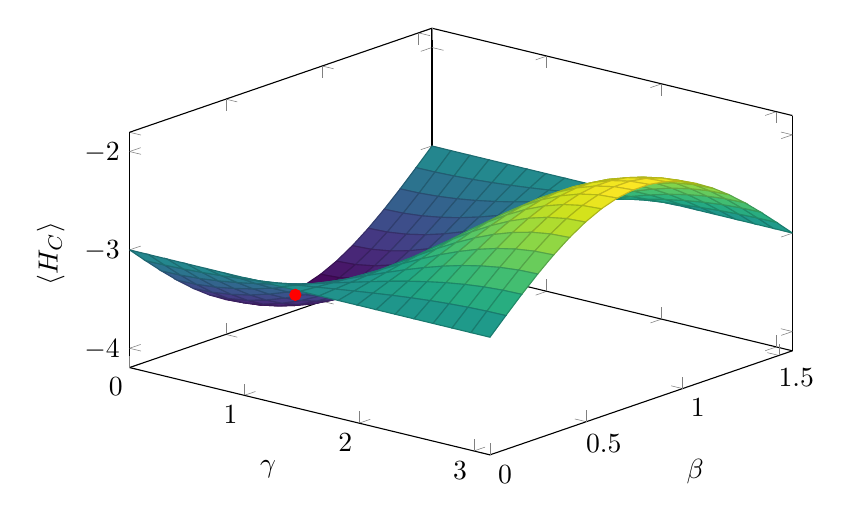
\begin{tikzpicture}
      \begin{axis}[
        width=10cm,
        height=7cm,
        xlabel=$\gamma$,
        ylabel=$\beta$,
        zlabel={$\langle H_C \rangle$},
        view={40}{30},
        colormap/viridis,
        ]

        \addplot3[
          surf,
          samples=20,
          domain=0:3.14,
          y domain=0:1.57,
          ]
          {-3 - cos(deg(x))*sin(deg(2*y))};

      % Optimal point
        \addplot3[only marks, mark=*, color=red] coordinates {(0.785, 0.393, -3.5)};
      \end{axis}
    \end{tikzpicture}
    \caption{Example landscape for \textsc{Max-Cut} QAOA with $P=1$ on a
    4-node cycle graph. The red dot indicates the optimal parameters.}
    \label{fig:landscape}
  \end{figure}
}

\vspace{0.3cm}

\index{Quantum Approximate Optimization Algorithms!Theoretical Insights}
\subsubsection*{Theoretical Insights for QAOA}

\noindent
\textbf{Adiabatic Quantum Computing Connection:}
\begin{itemize}
  \item As $P \to \infty$, QAOA approximates adiabatic quantum computing

  \item QAOA with optimal parameters can outperform the standard adiabatic
    algorithm

  \item For $P = poly(n)$, QAOA can capture quantum advantage for certain
    problems
\end{itemize}

\nt{
  The connection to adiabatic quantum computing suggests that QAOA can
  potentially solve NP-hard problems efficiently for specific instances,
  though this is not guaranteed in general.
}

\vspace{0.3cm}

\noindent
\textbf{Concentration of Parameters:}
\begin{itemize}
  \item For certain problems, optimal QAOA parameters concentrate (become
    instance-independent) as problem size grows

  \item This allows precomputing parameters for problem classes rather than
    instances

  \item Particularly relevant for local cost functions like \textsc{Max-Cut}
    on regular graphs
\end{itemize}

\ex{Parameter Concentration Example}{
  For \textsc{Max-Cut} on 3-regular graphs, optimal $\gamma$ and $\beta$
  values for $P=1$ are nearly identical across different random instances as
  the number of vertices increases. This means we can reuse the same
  parameters for any 3-regular graph without instance-specific optimization.
}

\begin{figure}[H]
  \centering
  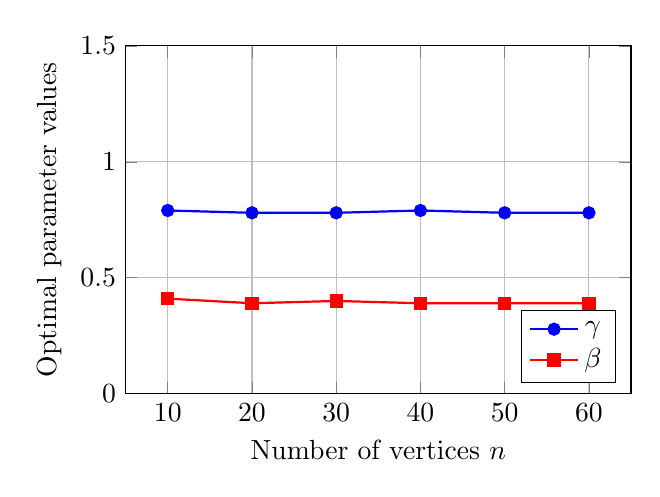
\begin{tikzpicture}
    \begin{axis}[
      width=8cm,
      height=6cm,
      xlabel={Number of vertices $n$},
      ylabel={Optimal parameter values},
      legend pos=south east,
      ymin=0, ymax=1.5,
      xtick={10, 20, 30, 40, 50, 60},
      grid=major
      ]

      \addplot[blue, mark=*, thick] coordinates {
        (10, 0.79)
        (20, 0.78)
        (30, 0.78)
        (40, 0.79)
        (50, 0.78)
        (60, 0.78)
      };

      \addplot[red, mark=square*, thick] coordinates {
        (10, 0.41)
        (20, 0.39)
        (30, 0.40)
        (40, 0.39)
        (50, 0.39)
        (60, 0.39)
      };

      \legend{$\gamma$, $\beta$}
    \end{axis}
  \end{tikzpicture}
  \caption{Parameter concentration for \textsc{Max-Cut} QAOA on 3-regular
  graphs}
  \label{fig:parameter-concentration}
\end{figure}


%%%%%%%%%%%%%%%%%%%%%%%%%%%%%%%%%%%%%%%%%%%%%%
% End of Lecture 14
%%%%%%%%%%%%%%%%%%%%%%%%%%%%%%%%%%%%%%%%%%%%%%

\section{Lecture 15: Wrapping Up QAOA: Intro to Coding in PennyLane,
QUBO}\label{sec:lecture15}

\subsection*{Review}

\qs{QAOA Circuit}{
  What are the main components of a QAOA circuit and how are they arranged?
}

\sol{
  A QAOA circuit consists of:
  \begin{enumerate}
    \item Initial state preparation: Apply Hadamard gates to create equal
      superposition $H^{\otimes n}|0\rangle^{\otimes n}$

    \item $P$ alternating layers of:
      \begin{itemize}
        \item Cost operator: $e^{-i\gamma_p H_C}$ which encodes the problem's
          objective function

        \item Mixer operator: $e^{-i\beta_p H_M}$ which explores the solution
          space
      \end{itemize}

    \item Final measurement in the computational basis
  \end{enumerate}
}

\vspace{0.3cm}

\index{Quantum Approximate Optimization Algorithms!PennyLane}
\subsection*{PennyLane}

\dfn{PennyLane}{PennyLane is an open-source software framework for quantum
  machine learning, quantum computing, and quantum chemistry. It enables users
  to train quantum circuits in the same way as neural networks, using automatic
differentiation techniques from machine learning.}

\vspace{0.3cm}

\noindent
\textbf{Key Features of PennyLane:}
\begin{itemize}
  \item \textbf{Hybrid quantum-classical computation}: Seamlessly connects
    classical machine learning libraries with quantum processing units

  \item \textbf{Automatic differentiation}: Computes gradients of quantum
    circuits for optimization tasks

  \item \textbf{Hardware agnostic}: Works with multiple quantum computing
    platforms and simulators

  \item \textbf{Built-in optimizers}: Includes various classical optimization
    algorithms

  \item \textbf{Quantum machine learning toolkit}: Provides implementations
    of common quantum algorithms and models
\end{itemize}

\begin{figure}[H]
  \centering
  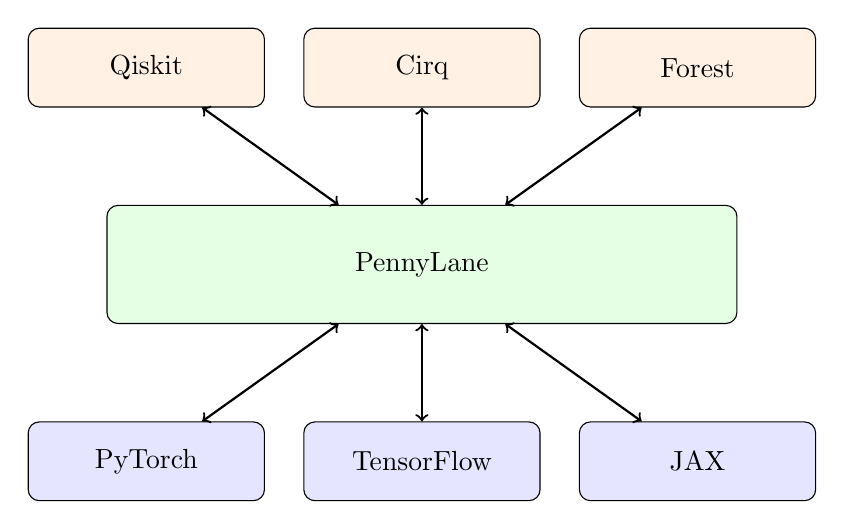
\begin{tikzpicture}
    \node[draw, rounded corners, fill=green!10, minimum width=8cm, minimum height=1.5cm] (pennylane) at (0,0) {PennyLane};

    \node[draw, rounded corners, fill=blue!10, minimum width=3cm, minimum height=1cm] (pytorch) at (-3.5,-2.5) {PyTorch};
    \node[draw, rounded corners, fill=blue!10, minimum width=3cm, minimum height=1cm] (tensorflow) at (0,-2.5) {TensorFlow};
    \node[draw, rounded corners, fill=blue!10, minimum width=3cm, minimum height=1cm] (jax) at (3.5,-2.5) {JAX};

    \node[draw, rounded corners, fill=orange!10, minimum width=3cm, minimum height=1cm] (qiskit) at (-3.5,2.5) {Qiskit};
    \node[draw, rounded corners, fill=orange!10, minimum width=3cm, minimum height=1cm] (cirq) at (0,2.5) {Cirq};
    \node[draw, rounded corners, fill=orange!10, minimum width=3cm, minimum height=1cm] (forest) at (3.5,2.5) {Forest};

    \draw[<->, thick] (pennylane) -- (pytorch);
    \draw[<->, thick] (pennylane) -- (tensorflow);
    \draw[<->, thick] (pennylane) -- (jax);

    \draw[<->, thick] (pennylane) -- (qiskit);
    \draw[<->, thick] (pennylane) -- (cirq);
    \draw[<->, thick] (pennylane) -- (forest);
  \end{tikzpicture}
  \caption{PennyLane connects classical ML frameworks with quantum computing
  platforms}
  \label{fig:pennylane-ecosystem}
\end{figure}

\vspace{0.3cm}

\noindent
\textbf{Basic Structure of a PennyLane Program:}
\begin{enumerate}
  \item Define a quantum device

  \item Create a quantum circuit using a QNode decorator

  \item Define a cost function

  \item Optimize the circuit parameters
\end{enumerate}

\begin{minted}{python}
  # Basic PennyLane workflow
  import pennylane as qml
  from pennylane import numpy as np

  # 1. Define a device
  dev = qml.device("default.qubit", wires=4)

  # 2. Define a quantum circuit (QNode)
  @qml.qnode(dev)
  def circuit(params):
  # Prepare initial state
  for i in range(4):
  qml.Hadamard(wires=i)

  # Apply parameterized gates
  qml.RX(params[0], wires=0)
  qml.RY(params[1], wires=1)

  # Return expectation values
  return qml.expval(qml.PauliZ(0))

  # 3. Run the circuit
  params = np.array([0.1, 0.2], requires_grad=True)
  result = circuit(params)
\end{minted}

\vspace{0.3cm}

\paragraph{QAOA Implementation in PennyLane} Here's how to implement QAOA for
MaxCut in PennyLane:

\begin{minted}{python}
  import pennylane as qml
  import networkx as nx
  from pennylane import numpy as np

  # Define the graph
  edges = [(0, 1), (0, 2), (0, 3), (1, 2), (2, 3)]
  graph = nx.Graph(edges)

  # Get the MaxCut cost and mixer Hamiltonians
  C, B = qml.qaoa.maxcut(graph)

  # Define the number of layers
  L = 1
  num_qubits = 4
  qubits = range(num_qubits)

  # Define the QAOA layers
  def qaoa_layer(gamma, beta):
  qml.qaoa.cost_layer(gamma, C)
  qml.qaoa.mixer_layer(beta, B)

  # Define the full circuit
  def circuit(params, **kwargs):
  for qubit in qubits:
  qml.Hadamard(wires=qubit)
  qml.layer(qaoa_layer, L, params[0], params[1])

  # Create a quantum device
  dev = qml.device("default.qubit", wires=qubits)

  # Define the cost function
  @qml.qnode(dev)
  def cost_function(params):
  circuit(params)
  return qml.expval(C)

  # Optimize the parameters
  optimizer = qml.AdagradOptimizer(stepsize=0.1)
  steps = 50
  params = np.array([[np.random.random()*2*np.pi],
  [np.random.random()*2*np.pi]],
  requires_grad=True)

  for i in range(steps):
  params = optimizer.step(cost_function, params)

  print("Optimal Cost:", cost_function(params))
  print("Optimal Parameters:", params)
\end{minted}


\nt{
  PennyLane's built-in QAOA module simplifies implementation by automatically
  constructing the cost and mixer Hamiltonians for problems like MaxCut. The
  \texttt{qml.layer} function is useful for applying repeated layers with
  different parameters.
}

\vspace{0.3cm}

\index{Quantum Approximate Optimization Algorithms!QUBO}
\subsection*{Quadratic Unconstrained Binary Optimization (QUBO)}

\dfn{Quadratic Unconstrained Binary Optimization (QUBO)}{
  \textbf{QUBO} is a mathematical optimization model involving binary
  variables with a quadratic objective function. It can be expressed as
  minimizing:

  \[
    f(\mathbf{x}) = \mathbf{x}^T Q \mathbf{x} = \sum_{i=1}^n \sum_{j=1}^n Q_{ij}x_i x_j
  \]

  where $\mathbf{x} \in \{0,1\}^n$ is a binary vector, and $Q$ is an $n
  \times n$ real-valued matrix representing the coefficients of the objective
  function.
}

\vspace{0.3cm}

\noindent
\textbf{QUBO Formulation:}
\begin{itemize}
  \item Linear terms: Represented on the diagonal of $Q$ ($Q_{ii}$)

  \item Quadratic terms: Represented on the off-diagonal elements of $Q$
    ($Q_{ij}$ where $i \neq j$)

  \item Can represent many NP-hard problems, including MaxCut, graph
    coloring, and traveling salesman problem
\end{itemize}

\vspace{0.3cm}

\ex{Job Priorities}{
  Consider a scheduling problem with 6 jobs ($J_0$ to $J_5$) where each job
  has a priority value $C_i$ and there are interference costs $I_{ij}$ if
  jobs $i$ and $j$ are scheduled together.

  \begin{itemize}
    \item Decision variables: $x_i = 1$ if job $i$ is selected, $0$ otherwise

    \item Priority values: $C_i$ represents the value of completing job $i$

    \item Interference costs: $I_{ij}$ represents the penalty if both jobs
      $i$ and $j$ are selected
  \end{itemize}

  The QUBO formulation is:
  \[
    \text{Maximize } f(x) = \sum_{i=0}^5 C_i x_i - \sum_{i=0}^5 \sum_{j>i}^5
    I_{ij} x_i x_j
  \]

  This can be rewritten in matrix form:
  \[
    f(x) = \mathbf{x}^T Q \mathbf{x}
  \]

  where $Q$ is a 6×6 matrix with:
  \begin{itemize}
    \item Diagonal elements $Q_{ii} = C_i$ (job priorities)

    \item Off-diagonal elements $Q_{ij} = -\frac{I_{ij}}{2}$ (interference
      costs)
  \end{itemize}

  For a QAOA implementation, we convert this to an Ising Hamiltonian by
  substituting $x_i = \frac{1 + s_i}{2}$, resulting in a Hamiltonian with
  $Z_i$ terms (for individual job priorities) and $Z_i Z_j$ terms (for job
  interferences).
}

\vspace{0.3cm}

\subsubsection*{QUBO in Code}

\begin{minted}{python}
import pennylane as qml
import numpy as np
import networkx as nx

# Define a QUBO problem
num_qubits = 6  # 6 jobs
np.random.seed(42)

# Generate random job priorities and interference costs
priorities = np.random.uniform(1, 10, size=num_qubits)
interferences = np.random.uniform(0, 5, size=(num_qubits, num_qubits))
interferences = (interferences + interferences.T) / 2  # Make symmetric
np.fill_diagonal(interferences, 0)  # No self-interference

# Create QUBO matrix
Q = np.zeros((num_qubits, num_qubits))
for i in range(num_qubits):
    Q[i, i] = priorities[i]  # Diagonal elements are priorities
    for j in range(num_qubits):
        if i != j:
            Q[i, j] = -interferences[i, j] / 2  # Off-diagonals are -interferences/2

# Convert QUBO to Ising Hamiltonian
def qubo_to_ising(Q):
    n = Q.shape[0]
    J = np.zeros((n, n))
    h = np.zeros(n)
    offset = 0

    for i in range(n):
        for j in range(n):
            if i == j:
                h[i] += Q[i, i] / 2
                offset += Q[i, i] / 4
            else:
                J[i, j] = Q[i, j] / 4
                h[i] += Q[i, j] / 4
                offset += Q[i, j] / 4

    return h, J, offset

h, J, offset = qubo_to_ising(Q)

# Create a PennyLane device
dev = qml.device("default.qubit", wires=range(num_qubits))

# Define the cost Hamiltonian operator
def cost_hamiltonian(h, J):
    obs = []
    # Single-qubit terms
    for i, coeff in enumerate(h):
        if abs(coeff) > 1e-10:
            obs.append(coeff * qml.PauliZ(i))

    # Two-qubit terms
    for i in range(num_qubits):
        for j in range(i+1, num_qubits):
            if abs(J[i, j]) > 1e-10:
                obs.append(J[i, j] * qml.PauliZ(i) @ qml.PauliZ(j))

    return qml.Hamiltonian(coeffs=[1.0] * len(obs), observables=obs)

# Create the cost Hamiltonian
H_C = cost_hamiltonian(h, J)

# Define the mixer Hamiltonian
H_M = qml.Hamiltonian(
    coeffs=[1.0] * num_qubits,
    observables=[qml.PauliX(i) for i in range(num_qubits)]
)

# Define the QAOA layers
def qaoa_layer(gamma, beta):
    qml.exp(H_C, gamma)
    qml.exp(H_M, beta)

# Define the QAOA circuit
@qml.qnode(dev)
def qaoa_circuit(params, p=1):
    # Initial state
    for i in range(num_qubits):
        qml.Hadamard(wires=i)

    # QAOA layers
    for i in range(p):
        qaoa_layer(params[2*i], params[2*i+1])

    # Return expectation value of the cost Hamiltonian
    return qml.expval(H_C)

# Optimize the QAOA parameters
p = 1  # Number of QAOA layers
params = np.random.uniform(0, 2*np.pi, size=2*p)
steps = 100
optimizer = qml.GradientDescentOptimizer(stepsize=0.1)

for i in range(steps):
    params = optimizer.step(lambda p: qaoa_circuit(p, p=p), params)
    if i % 10 == 0:
        cost = qaoa_circuit(params, p=p)
        print(f"Step {i}: Cost = {cost}")

# Final cost
final_cost = qaoa_circuit(params, p=p)
print(f"Final cost: {final_cost}")
print(f"Optimal parameters: {params}")

# Execute circuit with optimal parameters and measure in computational basis
@qml.qnode(dev)
def qaoa_measure(params, p=1):
    # Initial state
    for i in range(num_qubits):
        qml.Hadamard(wires=i)

    # QAOA layers
    for i in range(p):
        qaoa_layer(params[2*i], params[2*i+1])

    # Return samples in computational basis
    return qml.sample(wires=range(num_qubits))

# Get samples
n_samples = 1000
samples = qaoa_measure(params, p=p)
samples = np.array([samples for _ in range(n_samples)])

# Convert to binary solutions
binary_samples = (samples + 1) // 2  # Convert from {-1,1} to {0,1}

# Evaluate the original QUBO objective for each sample
def evaluate_qubo(x, Q):
    return x.T @ Q @ x

# Find the best solution
best_cost = float('inf')
best_solution = None
for sample in binary_samples:
    cost = evaluate_qubo(sample, Q)
    if cost < best_cost:
        best_cost = cost
        best_solution = sample

print(f"Best solution found: {best_solution}")
print(f"Best solution cost: {best_cost}")
\end{minted}

\vspace{0.3cm}

\nt{
  The code demonstrates converting a QUBO problem into an Ising Hamiltonian
  and solving it with QAOA in PennyLane. Key points:

  \begin{itemize}
    \item The job scheduling problem is transformed into a QUBO matrix $Q$

    \item The QUBO-to-Ising conversion involves a variable transformation
      from $x_i \in \{0,1\}$ to $s_i \in \{-1,+1\}$

    \item The Ising Hamiltonian has single-qubit $Z_i$ terms (from job
      priorities) and two-qubit $Z_i Z_j$ terms (from job interferences)

    \item The QAOA circuit alternates between problem Hamiltonian evolution
      and mixer Hamiltonian evolution

    \item Multiple samples are taken to find the best binary solution to the
      original problem
  \end{itemize}
}

\subsection*{Key Takeaways from QAOA Implementation}

\begin{itemize}
  \item QAOA is a versatile algorithm that can be applied to various
    combinatorial optimization problems

  \item The QUBO formulation provides a standardized approach to encode
    optimization problems for quantum algorithms

  \item PennyLane simplifies the implementation of quantum algorithms with
    its high-level abstractions and automatic differentiation

  \item The performance of QAOA depends on several factors:
    \begin{itemize}
      \item Number of layers ($p$)

      \item Choice of classical optimizer

      \item Initial parameter values

      \item Problem structure and size
    \end{itemize}

  \item QAOA represents a promising approach for quantum advantage in the
    NISQ era, especially for problems with efficient problem Hamiltonian
    implementations
\end{itemize}

\vspace{0.3cm}

\index{Quantum Approximate Optimization Algorithms!Applications}
\subsection*{Practical Considerations}

When implementing QAOA for real-world problems, consider:

\begin{itemize}
  \item \textbf{Problem encoding efficiency}: Different encodings may lead to
    circuits of varying depths and complexities

  \item \textbf{Parameter initialization}: Good initial parameters can
    significantly speed up convergence

  \item \textbf{Hardware constraints}: Consider connectivity limitations and
    noise characteristics of actual quantum hardware

  \item \textbf{Classical preprocessing}: Many problems benefit from
    classical preprocessing before quantum solving

  \item \textbf{Hybrid approaches}: Combining quantum and classical
    algorithms often yields the best results in practice
\end{itemize}

%%%%%%%%%%%%%%%%%%%%%%%%%%%%%%%%%%%%%%%%%%%%%%
% End of Lecture 15
%%%%%%%%%%%%%%%%%%%%%%%%%%%%%%%%%%%%%%%%%%%%%%



% ==============================
% PHASE IV: SPECIAL TOPICS
% ==============================
\chapter{Phase IV: Special Topics in Quantum Computing}

% ● Overview of quantum compilers and their role in quantum computing
% ● Introduction to quantum compiler optimizations
\section{Lecture 16: Quantum Compiler Optimizations}\label{sec:lecture16}

\subsection*{Review}

\qs{Number of $CX$ Gates}{
  How many $CX$ gates are required to implement the following QUBO cost function:

  \[
    c(x) = 0.1x_1x_2 + 0.0x_0x_2 + 0.2x_1x_2 + 0.3x_0x_1
  \]
}

\sol{
  To implement this QUBO cost function, we need to count the number of unique
  two-qubit interactions:

  \begin{itemize}
    \item $x_1x_2$: appears twice (0.1 and 0.2)
    \item $x_0x_1$: appears once (0.3)
    \item $x_0x_2$: appears once (0.0, but still requires a gate)
  \end{itemize}

  These interactions suggest 4 distinct $CX$ gates are required, noting that
  repeated interactions don't necessarily increase gate count.

  \[
    \boxed{4}
  \]
}

%%%%%%%%%%%%%%%%%%%%%%

% ● Overview of quantum compilers and their role in quantum computing
\index{quantum compilers}
\subsection*{Overview of Quantum Compilers}

Until now, we have primarily explored quantum algorithms through simulation
and theoretical models. However, translating these algorithms to actual
quantum hardware requires sophisticated compilation techniques. Quantum
compilers bridge the gap between theoretical quantum circuits and physical
quantum processors by addressing several key challenges:

\begin{itemize}
  \item \textbf{Hardware Constraints}: Different quantum hardware have
    varying gate sets, qubit connectivity, and noise characteristics

  \item \textbf{Circuit Optimization}: Reducing the number of gates and
    circuit depth to mitigate quantum decoherence

  \item \textbf{Error Mitigation}: Transforming circuits to be more resilient
    to quantum noise

  \item \textbf{Basis Gate Translation}: Converting high-level quantum gates
    to hardware-native gate sets
\end{itemize}

Compilers apply logical operations to optimize certain desirable metrics to make
the execution of a quantum circuit on quantum hardware more feasible, while
preserving the mathematical properties of the circuit.

Compilers for quantum circuits achieve this by two means-- reducing (1) the
number of gates, and (2) the circuit depth.

% ● Introduction to quantum compiler optimizations
\index{quantum compilers!optimizations}
\subsection*{Quantum Compiler Optimizations}

Quantum compiler optimizations can be categorized into several key strategies:

\paragraph{Gate Deletion}
Gate deletion is an optimization technique that removes quantum gates which
have no significant impact on the final quantum state. This can occur in
scenarios where:

\begin{itemize}
  \item Gates cancel each other out (e.g., $R_z(0)$ or successive rotations
    that net to zero)

  \item Gates act on qubits not involved in the final measurement

  \item Redundant gates can be eliminated without changing the circuit's
    computational outcome
\end{itemize}

\ex{Gate Deletion Example}{
Consider a circuit with successive rotations:

\[
  R_z(\pi/2) \circ R_z(-\pi/2) \equiv \text{Identity}
\]

A quantum compiler would recognize this and delete both gates, reducing
circuit complexity.
}


\paragraph{Gate Synthesis}
Gate synthesis involves combining multiple gates into more efficient,
hardware-compatible implementations. The primary goals are:

\begin{itemize}
  \item Reduce total gate count

  \item Minimize circuit depth

  \item Ensure compatibility with hardware gate sets
\end{itemize}

\ex{Gate Synthesis}{ Converting a three-qubit Toffoli gate into a sequence of
elementary $CX$ and single-qubit rotations that can be implemented on
hardware with limited multi-qubit gate capabilities. }


\paragraph{Gate Decomposition}
Gate decomposition breaks complex multi-qubit gates into sequences of
simpler, hardware-native gates. This is crucial because:

\begin{itemize}
  \item Quantum hardware often supports only limited gate types (e.g., $CX$,
    single-qubit rotations)

  \item Complex gates like Toffoli must be decomposed into supported
    primitive gates

  \item Decomposition helps manage qubit connectivity constraints
\end{itemize}

\ex{Toffoli Gate Decomposition}{
A Toffoli gate controlling on two qubits can be decomposed into a sequence of
$CX$ and single-qubit rotations:

\begin{enumerate}
  \item Reduce to controlled-$V$ gate

  \item Use ancilla qubits to implement multi-controlled rotations

  \item Minimize total gate count and depth
\end{enumerate}
}

\subsection*{Practical Implications}

The effectiveness of quantum compiler optimizations directly impacts:

\begin{itemize}
  \item \textbf{Circuit Fidelity}: Fewer gates mean less accumulated noise

  \item \textbf{Computational Efficiency}: Reduced gate count and depth

  \item \textbf{Hardware Utilization}: Better adaptation to specific quantum
    hardware constraints
\end{itemize}

\nt{Modern quantum compilers like Qiskit, Cirq, and PennyLane implement
sophisticated optimization passes that can dramatically reduce circuit
complexity before execution.}

%%%%%%%%%%%%%%%%%%%%%%%%%%%%%%%%%%%%%%%%%%%%%%
% End of Lecture 16
%%%%%%%%%%%%%%%%%%%%%%%%%%%%%%%%%%%%%%%%%%%%%%



% ● Architectural challenges and constraints in building quantum system
\section{Lecture 17: More on Quantum Compiler Optimizations, Quantum Computer
Architectures}\label{sec:lecture17}

\index{quantum compilers!optimizations}
\subsubsection*{More on Quantum Compiler Optimizations}

While our previous lecture explored gate deletion, synthesis, and
decomposition, gate commutativity represents another crucial optimization
technique. Not all quantum gates commute, but certain gate combinations can
be rearranged to improve circuit efficiency.

\paragraph{Gate Commutativity}
In quantum computing, gate commutativity refers to the ability to reorder
certain quantum gates without changing the final quantum state, enabling
compiler-level optimizations.

\begin{itemize}
  \item \textbf{Commutative Gates}: Some single-qubit gates, like $R_z$ and
    $R_x$, can be reordered

  \item \textbf{Non-Commutative Gates}: Controlled gates like $CX$ have
    strict ordering constraints

  \item \textbf{Optimization Strategies}:
    \begin{enumerate}
      \item Identify gates that can be safely reordered
      \item Minimize circuit depth
      \item Reduce gate interaction complexity
    \end{enumerate}
\end{itemize}

\ex{Gate Commutativity Example}{
  Consider two single-qubit rotations:

  \[
    R_z(\alpha) \circ R_x(\beta) \approx R_x(\beta) \circ R_z(\alpha)
  \]

  This property allows compilers to rearrange gates to optimize circuit
  structure.
}

\nt{Not all gate pairs commute. The non-commutativity of quantum gates is
fundamental to quantum computing's power and complexity.}


%%%%%%%%%%%%%%%%%


\index{superconducting qubit architectures}
\subsubsection*{Superconducting Qubit Architectures}

\dfn{Superconducting Qubit}{A quantum bit implemented using superconducting
  circuits, typically based on Josephson junctions, operating at extremely low
temperatures to maintain quantum coherence.}

\paragraph{Josephson Junction Fundamentals}
A Josephson junction is a key component in superconducting qubit design:

\begin{itemize}
  \item Consists of two superconductors separated by a thin insulating barrier
  \item Exhibits quantum tunneling of Cooper pairs
  \item Creates a nonlinear energy level structure crucial for qubit
    implementation
  \item Represented in circuit diagrams with an X symbol
\end{itemize}

\aside{
  \textbf{Why Are Quantum Computers Kept So Cold?}

  \vspace{0.3cm}

  Quantum computers require extreme cooling (millikelvin temperatures) to:

  \begin{itemize}
    \item Minimize thermal noise
    \item Preserve quantum coherence
    \item Reduce electron scattering
    \item Maintain superconducting properties
  \end{itemize}

  Typical operating temperatures are around 10-15 millikelvin, colder than
  outer space!
}

\subsubsection*{Frequency Management in Quantum Circuits}

\dfn{Detuning}{The deliberate offset of qubit operating frequencies to
prevent unwanted interactions and frequency collisions.}

Key challenges in superconducting qubit architectures:

\begin{itemize}
  \item \textbf{Frequency Collisions}: Qubits operating at similar
    frequencies can unintentionally couple

  \item \textbf{Detuning Strategies}:
    \begin{enumerate}
      \item Adjust individual qubit frequencies
      \item Create frequency separation
      \item Minimize cross-talk between qubits
    \end{enumerate}
\end{itemize}

\paragraph{Noise Effects in Quantum Computing}
Quantum computation is fundamentally challenged by two noise types:

\begin{itemize}
  \item \textbf{Coherent Noise}:
    \begin{itemize}
      \item Predictable and potentially controllable
      \item Minimized by reducing total 1 and 2-qubit gate operations
      \item Can be partially mitigated through precise gate implementations
    \end{itemize}

  \item \textbf{Non-Coherent Noise}:
    \begin{itemize}
      \item Unpredictable and harder to control
      \item Reduced by minimizing circuit depth
      \item Directly impacts the critical path of quantum computations
    \end{itemize}
\end{itemize}

\paragraph{Quantum State Decay and Measurement Challenges}
\begin{itemize}
  \item Quantum states naturally decay over time (decoherence)

  \item Measurement intrinsically disturbs quantum state

  \item Dynamical Decoupling (DD) techniques can help:
    \begin{itemize}
      \item Insertion of precise control pulses
      \item Attempts to cancel out environmental noise
      \item Extends quantum state coherence time
    \end{itemize}
\end{itemize}

\subsubsection*{Key Takeaways}

\begin{itemize}
  \item Quantum compiler optimizations extend beyond simple gate manipulation
  \item Superconducting qubits rely on complex physical mechanisms
  \item Noise management is critical in quantum computing architectures
  \item Frequency control and state preservation are fundamental challenges
\end{itemize}

%%%%%%%%%%%%%%%%%%%%%%%%%%%%%%%%%%%%%%%%%%%%%%
% End of Lecture 17
%%%%%%%%%%%%%%%%%%%%%%%%%%%%%%%%%%%%%%%%%%%%%%


\section{Lecture 18: Quantum Circuits as DAGs, Qubit Topologies, Logical to
Physical Mapping}\label{sec:lecture18}

\subsection*{Representing Quantum Circuits as Directed Acyclic Graphs (DAGs)}

Quantum circuits are complex, but they can be visualized as Directed Acyclic
Graphs (DAGs), where each gate is a node, and directed edges show which gates
must happen before others. This helps in understanding the circuit's flow and
dependencies.

\index{directed acyclic graph}
\dfn{Directed Acyclic Graph (DAG)}{
  A graph with directed edges and no cycles, used to represent a quantum
  circuit where:
  \begin{itemize}
    \item Nodes represent quantum gates or operations
    \item Directed edges indicate dependencies between gates (which
      operations must be performed before others)
    \item Time flows in the direction of the edges
    \item The acyclic property ensures no operation can depend on future
      operations
    \item Qubit lines from circuit diagrams become vertices at different time
      steps
    \item Two-qubit gates create edges between the affected qubits,
      establishing execution dependencies
  \end{itemize}

  This representation provides a mathematical foundation for analyzing
  circuit complexity, parallelism, and execution constraints.
}

\vspace{0.3cm}

\noindent
The conversion process from a standard quantum circuit to a DAG follows these
principles:

\begin{enumerate}
  \item Each quantum gate operation (single-qubit gates like \(H, X, R_x,
    R_y, R_z\) or two-qubit gates like CNOT, CZ) becomes a node in the graph.

  \item Directed edges connect a gate to all subsequent gates that depend on it:

    \begin{itemize}
      \item Gates acting on the same qubit(s) later in the circuit

      \item Two-qubit gates create dependencies between their control and
        target qubits
    \end{itemize}

  \item The resulting graph is inherently acyclic due to the temporal
    sequential nature of quantum circuits, with operations flowing forward in
    time without feedback loops.

  \item Gates that can be executed in parallel (acting on independent qubits)
    will not have dependency paths between them.
\end{enumerate}

This representation makes it clear which operations can be performed
simultaneously and which ones must wait for prior operations to complete.

\index{critical path}
\dfn{Critical Path}{
  The longest path through the circuit's DAG representation from input to
  output, which determines:

  \begin{itemize}
    \item The minimum execution time of the quantum circuit

    \item The sequence of dependent operations that cannot be parallelized

    \item The circuit depth when optimal parallelization is applied
  \end{itemize}

  The critical path is particularly important for quantum computing because:

  \begin{itemize}
    \item Quantum states are highly susceptible to decoherence over time

    \item Minimizing the critical path reduces the total time qubits must
      maintain coherence

    \item The number of two-qubit gates in the critical path often dominates
      error rates

    \item It provides a key metric for comparing different implementations of
      the same algorithm
  \end{itemize}
}

\vspace{0.3cm}

From the DAG, finding the critical path is a well-studied graph problem that
can be solved efficiently using topological sorting and dynamic programming
to compute the longest path length.

\subsection*{Different Current Qubit Topology Designs}

Where early qubit topology designs would potentially have some qubits with
up to 4 qubit connections, this proved to produce noise effects that would
cause incorrect output. Modern designs as of writing make use of altered
qubit topology layouts that have at most 3 connections to other qubits.

An interesting aspect is the fundamental trade-off between connectivity and
noise: more connections between qubits can enable faster computations with
fewer SWAP operations, but each additional coupling point introduces
potential sources of crosstalk and errors. This trade-off has led modern
designs to favor more conservative connectivity patterns that prioritize gate
fidelity over maximum connectivity.

This process of converting the circuit design onto actual, physical quantum
hardware is appropriately called \textbf{logical to physical mapping}.
Furthermore, the process seen in the above example where each qubit's path is
manifested in the physical circuit (potentially with the use of SWAP gates
due to the physical connections of the hardware) is called \textbf{routing}.

\vspace{0.3cm}

\index{logical to physical mapping}
\dfn{Logical $\rightarrow$ Physical Mapping}{
  The process of assigning logical qubits in a quantum algorithm to physical
  qubits on a quantum processor, considering:

  \begin{itemize}
    \item The hardware connectivity constraints of the physical device
    \item The specific interactions required by the quantum algorithm
    \item The quality and error rates of individual physical qubits
    \item The fidelity of two-qubit gate operations between specific physical
      qubits
  \end{itemize}

  Effective logical-to-physical mapping minimizes the number of additional
  operations (like SWAP gates) needed to execute the circuit on hardware with
  limited connectivity, which is crucial for reducing noise exposure and
  improving overall circuit performance.
}

\dfn{Routing}{
  The process of determining how to move quantum information between
  non-adjacent qubits on a quantum processor with limited connectivity,
  including:

  \begin{itemize}
    \item Inserting SWAP operations to move quantum states between physical
      qubits
    \item Determining the optimal sequence of SWAP operations to enable
      two-qubit gates between logical qubits mapped to non-adjacent physical
      qubits
    \item Balancing the trade-off between circuit depth increase and total
      gate count
    \item Considering the relative error rates of different physical
      connections when deciding routing paths
  \end{itemize}

  Efficient routing is critical for quantum circuit execution on NISQ (Noisy
  Intermediate-Scale Quantum) devices, as poor routing decisions can
  significantly degrade algorithm performance through accumulated errors.
}

\vspace{0.3cm}

As quantum devices continue to scale up, the complexity of the mapping and
routing problems grows significantly, making efficient compilation techniques
an essential area of research for practical quantum computing.

%%%%%%%%%%%%%%%%%%%%%%%%%%%%%%%%%%%%%%%%%%%%%%
% End of Lecture 18
%%%%%%%%%%%%%%%%%%%%%%%%%%%%%%%%%%%%%%%%%%%%%%



% ● More on Logical to Physical Mapping
\section{Lecture 19: More on Logical to Physical Mapping}\label{sec:lecture19}

We will continue to delve deeper into the process of mapping logical quantum
circuits to physical quantum hardware, focusing on IBM's heavy-hex lattice
topology. This mapping is a critical step in quantum computing due to the
constrained connectivity of physical qubits, often requiring the insertion of
SWAP gates to enable interactions between non-adjacent qubits. We will
explore how to decide on an effective mapping, and the consequences of
suboptimal choices on circuit efficiency. The IBM hardware operates with a
specific basis gate set—CX, X, RZ, and SX—into which all circuits must be
decomposed, adding another layer of complexity to the mapping process.

\subsubsection*{IBM's Heavy-Hex Lattice Topology}

IBM's quantum processors, such as those in the Falcon and Hummingbird
families, employ the heavy-hex lattice, a hexagonal arrangement of qubits
with additional edge qubits designed to minimize error rates. This topology
reduces frequency collisions and spectator errors compared to denser layouts
like square lattices, enhancing scalability and error correction
capabilities.\footnote{See \href{https://www.ibm.com/quantum/blog/heavy-hex-lattice}
{The IBM Quantum heavy hex lattice} for more details on the design motivation.}
For example, in a simplified seven-qubit heavy-hex layout, qubits might be
arranged as a chain (p0-p1-p2-p3-p4) with dangling qubits (p5 connected to
p1, p6 to p3), where each qubit has at most three neighbors.

\vspace{0.3cm}

\noindent
This connectivity can be represented conceptually as:

\begin{itemize}
  \item p0 -- p1 -- p2 -- p3 -- p4
  \item p5 -- p1
  \item p6 -- p3
\end{itemize}

\vspace{0.3cm}

\noindent
Such a structure balances connectivity with error mitigation, as explored in
research on topological codes.\footnote{Refer to \href{https://arxiv.org/abs/2404.15989}
{Creating entangled logical qubits in the heavy-hex lattice with topological
codes} for insights into error correction on this topology.}

\subsubsection*{Basis Gates and Hardware Constraints}

IBM's superconducting qubit platforms utilize a basis gate set consisting of
CX (CNOT), X, RZ, and SX gates. All logical circuits must be transpiled into
these gates for execution on IBM hardware.\footnote{Details on native gates
are available at \href{https://docs.quantum.ibm.com/guides/native-gates}{Native
gates and operations}.} This constraint, enforced by tools like Qiskit’s
transpiler, ensures compatibility but impacts circuit depth and fidelity. For
instance, a SWAP gate, necessary for non-adjacent qubit interactions,
decomposes into three CX gates, amplifying the importance of efficient mapping.

\ex{Mapping Logical Circuits to Physical Hardware}{

  Consider a simple logical circuit with a single CNOT gate between two qubits,
  q0 and q1:

  \[
    \begin{quantikz}
      \qw & \ctrl{1} & \qw \\
      \qw & \targ{} & \qw \\
    \end{quantikz}
  \]

  On a physical device with a linear topology (p0-p1-p2, where p0 is connected
  to p1, and p1 to p2), the mapping decision determines the circuit’s
  efficiency:

  \subsubsection*{Optimal Mapping}

  Map q0 to p0 and q1 to p1, where p0 and p1 are adjacent. The physical circuit
  remains:

  \[
    \begin{quantikz}
      \lstick{p0 (q0)} & \ctrl{1} & \qw \\
      \lstick{p1 (q1)} & \targ{} & \qw \\
      \lstick{p2} & \qw & \qw \\
    \end{quantikz}
  \]


  This requires no additional gates, preserving the circuit’s depth and
  minimizing error accumulation.

  \subsubsection*{Suboptimal Mapping}

  Map q0 to p0 and q1 to p2, where p0 and p2 are not directly connected. To
  execute the CNOT, we must swap q1 to an adjacent position:

  \begin{enumerate}
    \item SWAP p1 and p2 to move q1 to p1.
    \item Apply CNOT between p0 and p1.
    \item SWAP p1 and p2 back to restore the original mapping (if needed).
  \end{enumerate}

  The physical circuit becomes:

  \[
    \begin{quantikz}
      \lstick{p0 (q0)} & \qw & \qw & \ctrl{1} & \qw & \qw \\
      \lstick{p1} & \swap{1} & \qw & \targ{} & \swap{1} & \qw \\
      \lstick{p2 (q1)} & \swap{-1} & \qw & \qw & \swap{-1} & \qw \\
    \end{quantikz}
  \]

  Each SWAP decomposes into three CX gates, adding six CX gates total,
  significantly increasing depth and error potential.\footnote{For SWAP gate
    decomposition, see \href{https://learning.quantum.ibm.com/tutorial/explore-gates-and-circuits-with-the-quantum-composer}
  {Explore gates and circuits with IBM Quantum Composer}.}
}

\subsubsection*{Efficiency Impacts of Mapping Choices}

The choice of mapping directly affects circuit efficiency:

\begin{itemize}
  \item \textbf{Optimal Mapping:} No SWAPs, minimal gate count, and low error
    rate.
  \item \textbf{Suboptimal Mapping:} Two SWAPs, six additional CX gates,
    increased depth, and higher error probability due to more operations.
\end{itemize}

\vspace{0.3cm}

\noindent
For a larger circuit, such as one with three qubits (q0, q1, q2) and gates CX
q0 q1, CX q1 q2, CX q0 q2, mapping q0 to p0, q1 to p1, and q2 to p2 leverages
adjacency for the first two gates but requires a SWAP for the third (p0 to
p2). A better strategy might cluster frequently interacting qubits, reducing
SWAP overhead, as seen in optimization studies.\footnote{See
  \href{https://arxiv.org/html/2402.09705v1}{Linear Depth QFT over IBM
Heavy-hex Architecture} for mapping optimization techniques.}

\vspace{0.3cm}

\begin{center}
  \begin{table}[h]
    \centering
    \begin{tabular}{lcccc}
      \toprule
      Mapping Type & Number of SWAPs & Additional CNOTs & Circuit Depth Increase & Error Potential \\
      \midrule
      Optimal (Adjacent) & 0 & 0 & 0 & Low \\
      Suboptimal (Non-Adjacent) & 2 & 6 & Significant & High \\
      \bottomrule
    \end{tabular}
    \caption{Comparison of mapping efficiency for a two-qubit CNOT circuit.}
  \end{table}
\end{center}

\ex{Larger Circuit Mapping Example}{

  Consider a three-qubit logical circuit:

  \[
    \begin{quantikz}
      \lstick{q0} & \ctrl{1} & \qw & \ctrl{2} & \qw \\
      \lstick{q1} & \targ{} & \ctrl{1} & \qw & \qw \\
      \lstick{q2} & \qw & \targ{} & \targ{} & \qw \\
    \end{quantikz}
  \]


  On a heavy-hex segment (p0-p1-p2), an optimal mapping (q0 to p0, q1 to p1, q2
  to p2) executes the first two gates directly but requires a SWAP for CX q0 q2:

  \[
    \begin{quantikz}
      \lstick{p0 (q0)} & \ctrl{1} & \qw & \qw & \ctrl{1} & \qw \\
      \lstick{p1 (q1)} & \targ{} & \ctrl{1} & \swap{1} & \targ{} & \qw \\
      \lstick{p2 (q2)} & \qw & \targ{} & \swap{-1} & \targ{} & \qw \\
    \end{quantikz}
  \]

  Here, the SWAP p1 p2 moves q2 to p1, allowing the CNOT, adding three CX
  gates. A suboptimal mapping (e.g., q0 to p0, q1 to p2, q2 to p1) would
  require multiple SWAPs, worsening efficiency.
}

\subsubsection*{Practical Implications}

Efficient mapping is crucial for quantum algorithm performance, especially as
hardware scales to larger qubit counts (e.g., IBM’s Crossbill with 408
qubits).\footnote{See \href{https://www.ibm.com/quantum/blog/ibm-quantum-roadmap-2025}
{IBM roadmap to quantum-centric supercomputers} for future hardware plans.}
Suboptimal mappings can render circuits impractical due to excessive depth,
while optimal mappings, guided by tools like Qiskit, enhance fidelity.\footnote{
  For hardware-aware strategies, see \href{https://www.ibm.com/blogs/research/2020/09/hardware-aware-quantum/}
{Hardware-aware approach for fault-tolerant quantum computation}.}

%%%%%%%%%%%%%%%%%%%%%%%%%%%%%%%%%%%%%%%%%%%%%%
% End of Lecture 19
%%%%%%%%%%%%%%%%%%%%%%%%%%%%%%%%%%%%%%%%%%%%%%



% ● Quantum error correction
\section{Lecture 20: Quantum Error Correction-- Bit Flip Errors}
\label{sec:lecture20}

Quantum circuits are highly sensitive to errors due to decoherence and
environmental noise, making error correction a cornerstone of reliable
quantum computation. This sensitivity stems from qubits losing their quantum
state through interactions with the environment, a process known as
decoherence. In quantum computing, significant effort is devoted not only to
compiler optimizations that reduce circuit depth but also to creating
redundancies within quantum circuits to protect information and enable
fault-tolerant computation.\footnote{For an overview, see
  \href{https://q-ctrl.com/topics/what-is-quantum-error-correction}{What is
quantum error correction?}} This lecture contrasts classical error correction
with quantum approaches, highlighting the unique challenges posed by quantum
mechanics.

\index{error correction!classical error detection}
\subsection*{Classical Error Correction}

Classical bits, which can be either 0 or 1, are prone to errors with a
probability \( p \in [0, 1] \), where the bit flips with probability \( p \)
and remains correct with probability \( 1 - p \). This is formally expressed as:

\[
  b =
  \begin{cases}
    \text{correct}, & \text{with probability } 1 - p \\
    \text{incorrect}, & \text{with probability } p
  \end{cases}
\]

Classical bits typically experience only bit-flip errors (e.g., 0 to 1 or 1
to 0), unlike quantum bits, which can also suffer phase flips due to their
superposition and entanglement properties.

\ex{Error Encoding of 3 for Classical Bit}{
  Suppose \( b = 0 \). Classically, we can build redundancies by making three
  copies of \( b \), sending \( 000 \), and taking a majority vote at the
  receiver to decode the original bit. The possible received states, their
  probabilities, and the decoded outcomes are shown in the table below:

  \begin{table}[H]
    \centering
    \begin{tabular}{lccc}
      \toprule
      Received State & Probability & Decoded Value & Correct? \\
      \midrule
      000 & \( (1 - p)^3 \) & 0 & Yes \\
      001 & \( (1 - p)^2 p \) & 0 & Yes \\
      010 & \( (1 - p)^2 p \) & 0 & Yes \\
      100 & \( (1 - p)^2 p \) & 0 & Yes \\
      011 & \( (1 - p) p^2 \) & 1 & No \\
      101 & \( (1 - p) p^2 \) & 1 & No \\
      110 & \( (1 - p) p^2 \) & 1 & No \\
      111 & \( p^3 \) & 1 & No \\
      \bottomrule
    \end{tabular}
    \caption{Probabilities of received states for a 3-bit repetition code.}
  \end{table}

  \vspace{0.3cm}

  The probability of correctly decoding \( b = 0 \) is the sum of
  probabilities where the majority is 0: \( (1 - p)^3 + 3 (1 - p)^2 p = 1 -
  3p^2 + 2p^3 \). This improves the success probability from the initial \( 1
  - p \) to \( 1 - 3p^2 + 2p^3 \).

  \vspace{0.3cm}

  For \( p = 0.01 \), the initial success rate without encoding is 0.99, but
  with three-bit redundancy, it increases to 0.999702, significantly
  enhancing reliability.
}

\vspace{0.3cm}

Interestingly, modern devices like smart phones employ similar redundancy
techniques, often using 5-7 redundancy bits in flash memory for error
correction. This contributes to power consumption due to the additional
storage and processing required, a trade-off for improved data integrity in
noisy environments.

\vspace{0.3cm}

\index{error correction!quantum error detection}
\subsection*{Qubit Flip Error Correction}
Quantum error correction is fundamentally more complex than its classical
counterpart due to the no-cloning theorem, which states that an unknown
quantum state cannot be perfectly copied.\footnote{For details on the
no-cloning theorem, see \href{https://learning.quantum.ibm.com/course/basics-of-quantum-information/quantum-circuits}{Quantum circuits}.}
This prevents us from simply making trivial copies of a qubit’s state, as in
classical systems. Even attempting to "clone" a qubit would not preserve the
original superposition \( |\psi\rangle = \alpha |0\rangle + \beta |1\rangle
\), rendering direct repetition impractical. Instead, quantum error
correction relies on encoding logical qubits into entangled states across
multiple physical qubits, using codes like the repetition code.

\vspace{0.3cm}

\index{error correction!repetition code}
\dfn{Repetition Code}{
  The quantum \textbf{repetition code} encodes a single logical qubit into
  multiple physical qubits to protect against errors. For a code distance of
  3, the state \( |\psi\rangle = \alpha |0\rangle + \beta |1\rangle \) is
  encoded into \( |\psi_3\rangle = \alpha |000\rangle + \beta |111\rangle \).
  This is achieved by starting with the initial qubit in \( |\psi\rangle \)
  and two ancilla qubits in \( |0\rangle \), then applying CNOT gates from
  the original qubit to the ancillas:

  \[
    \begin{quantikz}
      \lstick{$q_0 \: \ket{\psi}$} & \ctrl{1} & \ctrl{2} & \qw \\
      \lstick{$q_1 : \zero$} & \targ{} & \qw & \qw \\
      \lstick{$q_2 : \zero$} & \qw & \targ{} & \qw \\
    \end{quantikz}
  \]

  This circuit entangles the qubits such that a single bit-flip error (e.g.,
  \( X \) on one qubit) can be detected and corrected using syndrome
  measurements without collapsing the superposition.\footnote{See
    \href{https://www.nature.com/articles/s41567-023-02282-2}{Protecting
    expressive circuits with a quantum error detection code} for encoding
  techniques.}
}

\index{error correction!syndrome}
\dfn{Syndrome}{
  In quantum computing, \textbf{syndrome} measurement is a process used in
  quantum error correction (QEC) to identify errors without revealing the
  quantum information stored in the qubits. The syndrome measurement provides
  information about the type of error that has occurred, such as a bit flip
  or a phase flip, but it does not reveal the information stored in the
  logical qubit, thus preserving quantum superposition
}

\vspace{0.3cm}

To correct a single qubit flip error, consider the encoded state \(
|\psi_3\rangle = \alpha \ket{000} + \beta \ket{111} \). If an \( X \)
error occurs on \( q_1 \), the state becomes \( \alpha \ket{010} + \beta
\ket{101} \). Syndrome measurements are performed using two ancilla qubits
to measure the parities \( q_0 q_1 \) and \( q_1 q_2 \):

\begin{itemize}
  \item Measure \( X \otimes X \) between \( q_0 \) and \( q_1 \) with an
    ancilla initialized in \( |+\rangle \), applying CNOTs from \( q_0 \) and
    \( q_1 \) to the ancilla, then measuring it in the \( Z \)-basis. Outcome
    -1 indicates a flip on \( q_0 \) or \( q_1 \).
  \item Measure \( X \otimes X \) between \( q_1 \) and \( q_2 \) similarly.
    Outcome -1 indicates a flip on \( q_1 \) or \( q_2 \).
\end{itemize}

\vspace{0.3cm}

\noindent
For the error on \( q_1 \):
\begin{itemize}
  \item \( q_0 q_1 \): -1 (flip detected).
  \item \( q_1 q_2 \): -1 (flip detected).
  \item Syndrome (-1, -1) uniquely identifies \( q_1 \), and an \( X \) gate
    corrects it, restoring \( |\psi_3\rangle \).
\end{itemize}

This process, detailed in \href{https://www.ibm.com/quantum/blog/error-correction-codes}
{Error correcting codes for near-term quantum computers}, ensures correction
without measuring the logical state directly, preserving quantum information.

\aside{
  \textbf{Silent Data Corruption (SDC)} occurs when errors go undetected,
  posing significant risks in computing systems. In classical systems, SDC
  can corrupt data silently, leading to integrity issues in storage or
  processing. In quantum computing, undetected errors can propagate through
  entanglements, undermining computation reliability and producing incorrect
  results. This is particularly challenging due to the fragility of quantum
  states, making robust error correction essential to mitigate SDC and
  achieve fault tolerance.\footnote{See
    \href{https://physicsworld.com/a/why-error-correction-is-quantum-computings-defining-challenge}{Why
    error correction is quantum computing's defining challenge} for SDC
  implications.}
}

%%%%%%%%%%%%%%%%%%%%%%%%%%%%%%%%%%%%%%%%%%%%%%
% End of Lecture 20
%%%%%%%%%%%%%%%%%%%%%%%%%%%%%%%%%%%%%%%%%%%%%%



% ==============================
% PHASE V: CONCLUDING LECTURES
% ==============================
% \chapter{Phase V: Concluding Lectures}
% LECTURES TBD

% ==============================
% QUICK REFERENCE
% ==============================
\chapter{Quantum Computing Quick Reference}
\section{Cheatsheet}\label{sec:cheatsheet}

% Local formatting for the cheatsheet
\begingroup
\setlength{\parindent}{0pt}
\setlength{\parskip}{0pt plus 0.5ex}
\raggedright
\footnotesize

\makeatother

\begin{multicols}{3}

  \section*{Linear Algebra Notation}
  \begin{itemize}[leftmargin=*,nosep,topsep=0pt]
    \item \textbf{Bra-Ket}: Ket $|\psi\rangle = \begin{bmatrix} \alpha \\
      \beta \end{bmatrix}$, Bra $\langle\psi| = [\alpha^* \; \beta^*]$

    \item \textbf{Inner Product}: $\langle\phi|\psi\rangle = \phi^\dagger\psi
      = \sum_i \phi_i^*\psi_i$

    \item \textbf{Norm}: $\|\psi\|^2 = \langle\psi|\psi\rangle = \sum_i
      |\psi_i|^2$

    \item \textbf{Outer Product}: $|\psi\rangle\langle\phi| = \begin{bmatrix}
        \psi_1\phi_1^* & \psi_1\phi_2^* \\ \psi_2\phi_1^* & \psi_2\phi_2^*
      \end{bmatrix}$

    \item \textbf{Tensor Product}: $|\psi\rangle \otimes |\phi\rangle =
      \begin{bmatrix} \psi_1\phi_1 \\ \psi_1\phi_2 \\ \psi_2\phi_1 \\
      \psi_2\phi_2 \end{bmatrix}$

    \item \textbf{Matrix Mult}: $(AB)_{ij} = \sum_k A_{ik}B_{kj}$

    \item \textbf{Unitary}: $U^\dagger U = UU^\dagger = I$, preserves norms
      and inner products

    \item \textbf{Hermitian}: $H = H^\dagger$, eigenvalues are real

    \item \textbf{Magnitude}: Real: $\|v\| = \sqrt{\sum_i v_i^2}$, Complex:
      $\|v\| = \sqrt{\sum_i |v_i|^2}$

  \end{itemize}

  \conceptbox{Important Property}{Tensor products are \textit{not commutative}:
  $A \otimes B \neq B \otimes A$ generally}

  \section*{Qubit Representation}
  \begin{itemize}[leftmargin=*,nosep,topsep=0pt]
    \item \textbf{Dirac Notation}: $|\psi\rangle = \alpha|0\rangle +
      \beta|1\rangle$, where $\alpha,\beta \in \mathbb{C}$ and $|\alpha|^2 +
      |\beta|^2 = 1$

    \item \textbf{Computational Basis}: $|0\rangle = \begin{bmatrix} 1 \\ 0
        \end{bmatrix}$, $|1\rangle = \begin{bmatrix} 0 \\ 1 \end{bmatrix}$
    \end{itemize}

    \section*{Universal Bases}
    \begin{itemize}[leftmargin=*,nosep,topsep=0pt]
      \item \textbf{Computational}: $\{|0\rangle, |1\rangle\}$ \\
        $(\theta=0, \phi=0; \theta=\pi, \phi=0)$

      \item \textbf{Hadamard}: $\{|+\rangle, |-\rangle\}$ where\\
        $|+\rangle = \frac{1}{\sqrt{2}}(|0\rangle + |1\rangle)$\\
        $|-\rangle = \frac{1}{\sqrt{2}}(|0\rangle - |1\rangle)$\\
        $(\theta=\frac{\pi}{2}, \phi=0; \theta=\frac{\pi}{2}, \phi=\pi)$

      \item \textbf{Phase}: $\{|+i\rangle, |-i\rangle\}$ where\\
        $|+i\rangle = \frac{1}{\sqrt{2}}(|0\rangle + i|1\rangle)$\\
        $|-i\rangle = \frac{1}{\sqrt{2}}(|0\rangle - i|1\rangle)$\\
        $(\theta=\frac{\pi}{2}, \phi=\frac{\pi}{2}; \theta=\frac{\pi}{2},
        \phi=-\frac{\pi}{2})$
    \end{itemize}

    \section*{Bloch Sphere}
    \begin{itemize}[leftmargin=*,nosep,topsep=0pt]
      \item \textbf{Equation}: $|\psi\rangle = \cos\frac{\theta}{2}|0\rangle +
        e^{i\phi}\sin\frac{\theta}{2}|1\rangle$\\
        where $\theta \in [0,\pi]$, $\phi \in [0,2\pi)$

      \item \textbf{Cartesian Projection}:
        \begin{align*}
          x &= \sin\theta\cos\phi\\
          y &= \sin\theta\sin\phi\\
          z &= \cos\theta
        \end{align*}

    \end{itemize}

    \section*{Quantum Measurement}
    \begin{itemize}[leftmargin=*,nosep,topsep=0pt]
      \item \textbf{Probability}: For measuring state $|\psi\rangle$ in basis
        $|b\rangle$:
        \begin{align*}
          P(b) = |\langle b|\psi\rangle|^2
        \end{align*}

      \item \textbf{Post-measurement state}:
        \begin{align*}
          |\psi_{\text{new}}\rangle = \frac{|b\rangle\langle
          b|\psi\rangle}{\sqrt{P(b)}}
        \end{align*}

      \item For $|\psi\rangle = \alpha|0\rangle + \beta|1\rangle$:
        \begin{align*}
          P(0) = |\alpha|^2, \quad P(1) = |\beta|^2
        \end{align*}

    \end{itemize}

    \section*{Single-Qubit Gates}
    \begin{itemize}[leftmargin=*,nosep,topsep=0pt]
      \item \textbf{Properties}:
        \begin{itemize}[nosep]
          \item Reversible: $U^\dagger U = UU^\dagger = I$

          \item Preserve norm: $\|U|\psi\rangle\| = \||\psi\rangle\|$

          \item Linear: $U(\alpha|\psi\rangle + \beta|\phi\rangle) = \alpha
            U|\psi\rangle + \beta U|\phi\rangle$

        \end{itemize}
    \end{itemize}

    \section*{Pauli Gates}
    \begin{itemize}[leftmargin=*,nosep,topsep=0pt]
      \item \textbf{Pauli-X (NOT)}: $X = \begin{bmatrix} 0 & 1 \\ 1 & 0
        \end{bmatrix}$
        \begin{itemize}[nosep]
          \item $X|0\rangle = |1\rangle$, $X|1\rangle = |0\rangle$
          \item $X|+\rangle = |+\rangle$, $X|-\rangle = -|-\rangle$
        \end{itemize}

        \item \textbf{Pauli-Y}: $Y = \begin{bmatrix} 0 & -i \\ i & 0 \end{bmatrix}$
          \begin{itemize}[nosep]
            \item $Y|0\rangle = i|1\rangle$, $Y|1\rangle = -i|0\rangle$
          \end{itemize}

        \item \textbf{Pauli-Z (Phase Flip)}: $Z = \begin{bmatrix} 1 & 0 \\ 0 & -1
          \end{bmatrix}$
          \begin{itemize}[nosep]
            \item $Z|0\rangle = |0\rangle$, $Z|1\rangle = -|1\rangle$
            \item $Z|+\rangle = |-\rangle$, $Z|-\rangle = |+\rangle$
          \end{itemize}
        \end{itemize}

        \section*{Rotation Gates}
        \begin{itemize}[leftmargin=*,nosep,topsep=0pt]
          \item \textbf{X-rotation}: $R_X(\theta) = e^{-i\theta X/2} =
            \begin{bmatrix} \cos\frac{\theta}{2} & -i\sin\frac{\theta}{2} \\
            -i\sin\frac{\theta}{2} & \cos\frac{\theta}{2} \end{bmatrix}$

          \item \textbf{Y-rotation}: $R_Y(\theta) = e^{-i\theta Y/2} =
              \begin{bmatrix} \cos\frac{\theta}{2} & -\sin\frac{\theta}{2} \\
              \sin\frac{\theta}{2} & \cos\frac{\theta}{2} \end{bmatrix}$

            \item \textbf{Z-rotation}: $R_Z(\theta) = e^{-i\theta Z/2} =
                \begin{bmatrix} e^{-i\theta/2} & 0 \\ 0 & e^{i\theta/2} \end{bmatrix}$
            \end{itemize}

            \section*{Other Important Gates}
            \begin{itemize}[leftmargin=*,nosep,topsep=0pt]
              \item \textbf{Hadamard}: $H = \frac{1}{\sqrt{2}}\begin{bmatrix} 1 & 1 \\
                1 & -1 \end{bmatrix}$
                \begin{itemize}[nosep]
                  \item $H|0\rangle = |+\rangle$, $H|1\rangle = |-\rangle$

                  \item $H|+\rangle = |0\rangle$, $H|-\rangle = |1\rangle$

                  \item $H^2 = I$
                \end{itemize}

                \item \textbf{Phase (S)}: $S = \begin{bmatrix} 1 & 0 \\ 0 & i \end{bmatrix}$
                  \begin{itemize}[nosep]
                    \item $S|+\rangle = |+i\rangle = \frac{1}{\sqrt{2}}(|0\rangle +
                      i|1\rangle)$

                    \item $S^2 = Z$
                  \end{itemize}

                \item \textbf{T Gate}: $T = \begin{bmatrix} 1 & 0 \\ 0 & e^{i\pi/4}
                  \end{bmatrix}$
                  \begin{itemize}[nosep]
                    \item $T|+\rangle = \frac{1}{\sqrt{2}}(|0\rangle + e^{i\pi/4}|1\rangle)$
                    \item $T^2 = S$, $T^4 = Z$
                  \end{itemize}

                  \item \textbf{General Phase}: $P(\theta) = \begin{bmatrix} 1 & 0 \\ 0 &
                    e^{i\theta} \end{bmatrix}$
                    \begin{itemize}[nosep]
                      \item $S = P(\pi/2)$, $T = P(\pi/4)$, $Z = P(\pi)$
                    \end{itemize}
                  \end{itemize}

                  \section*{Circuit Notation}
                  \begin{itemize}[leftmargin=*,nosep,topsep=0pt]
                    \item \textbf{Elements}:
                      \begin{itemize}[nosep]
                        \item Qubit: Horizontal line
                        \item Gates: Boxes with labels
                        \item Measurement: Meter symbol (if available)
                        \item Time: Left $\to$ Right
                        \item Controlled operations: Vertical line with dot
                        \item Control on $|1\rangle$: Filled dot $\bullet$
                        \item Control on $|0\rangle$: Empty dot $\circ$
                        \item Endiannes: Top (MSB) $\to$ Bottom (LSB)
                      \end{itemize}
                  \end{itemize}
                  \conceptbox{Important}{Matrix order in circuit is opposite to
                    mathematical notation:

                    $U_1 U_2$ in circuit $=$ $U_2 U_1$ in matrix form
                  }

                  \section*{Multi-Qubit Gates}
                  \begin{itemize}[leftmargin=*,nosep,topsep=0pt]
                    \item \textbf{CNOT} (Controlled-NOT):
                      \begin{align*}
                        \text{CNOT} = \begin{bmatrix}
                          1 & 0 & 0 & 0 \\
                          0 & 1 & 0 & 0 \\
                          0 & 0 & 0 & 1 \\
                          0 & 0 & 1 & 0
                        \end{bmatrix}
                      \end{align*}
                      \begin{itemize}[nosep]
                        \item Effect: $|c,t\rangle \rightarrow |c, t \oplus c\rangle$
                        \item $|00\rangle \to |00\rangle$, $|01\rangle \to |01\rangle$
                        \item $|10\rangle \to |11\rangle$, $|11\rangle \to |10\rangle$
                      \end{itemize}

                    \item \textbf{Controlled-Z}:
                      \begin{align*}
                        \text{CZ} = \begin{bmatrix}
                          1 & 0 & 0 & 0 \\
                          0 & 1 & 0 & 0 \\
                          0 & 0 & 1 & 0 \\
                          0 & 0 & 0 & -1
                        \end{bmatrix}
                      \end{align*}
                      \begin{itemize}[nosep]
                        \item Effect: $|x,y\rangle \to (-1)^{xy}|x,y\rangle$
                        \item Only changes $|11\rangle \to -|11\rangle$
                        \item Symmetric: Either qubit can be control
                      \end{itemize}

                    \item \textbf{Toffoli} (CCNOT):
                      \begin{itemize}[nosep]
                        \item Effect: $|x,y,z\rangle \to |x,y,z \oplus (x \cdot y)\rangle$
                        \item Flips target only if both controls are $|1\rangle$
                      \end{itemize}

                    \item \textbf{SWAP}:
                      \begin{align*}
                        \text{SWAP} = \begin{bmatrix}
                          1 & 0 & 0 & 0 \\
                          0 & 0 & 1 & 0 \\
                          0 & 1 & 0 & 0 \\
                          0 & 0 & 0 & 1
                        \end{bmatrix}
                      \end{align*}
                      \begin{itemize}[nosep]
                        \item Effect: $|a,b\rangle \to |b,a\rangle$

                        \item Implementation: $\text{CNOT}_{1,2} \cdot \text{CNOT}_{2,1}
                          \cdot \text{CNOT}_{1,2}$
                      \end{itemize}

                    \item \textbf{Flipped CNOT}:
                      \begin{align*}
                        (H \otimes H) \cdot \text{CNOT} \cdot (H \otimes H) = \begin{bmatrix}
                          1 & 0 & 0 & 0 \\
                          0 & 0 & 0 & 1 \\
                          0 & 0 & 1 & 0 \\
                          0 & 1 & 0 & 0
                        \end{bmatrix}
                      \end{align*}
                  \end{itemize}

                  \section*{Key Quantum Properties}
                  \begin{itemize}[leftmargin=*,nosep,topsep=0pt]
                    \item \textbf{Reversibility}: All quantum gates are reversible
                      \begin{itemize}[nosep]
                        \item To reverse a circuit, apply $U^\dagger$ gates in reverse order
                      \end{itemize}

                    \item \textbf{No-Cloning Theorem}: Cannot create an identical copy of an
                      unknown quantum state
                      \begin{align*}
                        \nexists U: U(|\psi\rangle \otimes |0\rangle) = |\psi\rangle \otimes
                        |\psi\rangle
                      \end{align*}

                    \item \textbf{Entanglement}: States that cannot be factored as tensor
                      products of individual states
                      \begin{itemize}[nosep]
                        \item E.g., Bell state: $\frac{1}{\sqrt{2}}(|00\rangle + |11\rangle)$
                      \end{itemize}
                  \end{itemize}

                  \section*{Bell Pair}
                  \begin{itemize}[leftmargin=*,nosep,topsep=0pt]
                    \item \textbf{Bell States} (maximally entangled):
                      \begin{align*}
                        |\Phi^+\rangle &= \frac{1}{\sqrt{2}}(|00\rangle + |11\rangle)\\
                        |\Phi^-\rangle &= \frac{1}{\sqrt{2}}(|00\rangle - |11\rangle)\\
                        |\Psi^+\rangle &= \frac{1}{\sqrt{2}}(|01\rangle + |10\rangle)\\
                        |\Psi^-\rangle &= \frac{1}{\sqrt{2}}(|01\rangle - |10\rangle)
                      \end{align*}

                    \item Bell-Pair Circuit
                      \[
                        \begin{quantikz}
                          q_1 \quad \lstick{$\zero$} & \gate{H} & \ctrl{1} & \meter{} \\
                          q_0 \quad \lstick{$\zero$} & \qw & \gate{X} & \qw \\
                        \end{quantikz}
                      \]
                  \end{itemize}

                  \section*{Grover's Algorithm}
                  \begin{itemize}[leftmargin=*,nosep,topsep=0pt]
                    \item \textbf{Purpose}: Search unstructured database of $N$ items in
                      $O(\sqrt{N})$ time

                    \item \textbf{Algorithm}:
                      \begin{enumerate}[nosep]
                        \item Initialize: $|s\rangle = H^{\otimes n}|0\rangle^{\otimes n}$
                        \item Repeat $O(\sqrt{N})$ times:
                          \begin{itemize}[nosep]
                            \item Oracle ($O$): $O|x\rangle = (-1)^{f(x)}|x\rangle$ where
                              $f(x)=1$ for solution

                            \item Diffusion ($D$): $D = 2|s\rangle\langle s| - I$
                          \end{itemize}

                        \item Measure to find solution with high probability
                      \end{enumerate}

                      \conceptbox{Important Insight}{Grover's algorithm
                        provides quadratic speedup over classical search, which
                      is proven to be optimal for quantum algorithms}

                    \item \textbf{Circuit}
                      \[
                        \resizebox{0.25\textwidth}{!}{
                          \begin{quantikz}
                            \lstick{$q_{n - 1}$} & \gate{H} & \gate[5]{\shortstack{$f(x)$ \\ Oracle}} & \qw & \gate[5]{\text{Diffusion Circuit}} & \meter{} \\
                            \lstick{$q_{n - 2}$} & \gate{H} & & & & \meter{} \\
                            \vdots & \vdots & & \vdots & & \vdots \\
                            \lstick{$q_1$} & \gate{H} & & & & \meter{} \\
                            \lstick{$q_0$} & \gate{H} & & & & \meter{}
                          \end{quantikz}
                        }
                      \]

                      \[
                        \hspace{1cm}
                        \underbrace{\hspace{3cm}}_{\text{Repeat } \sqrt{2^n} \text{ times}}
                      \]

                    \item \textbf{General Diffusion Circuit}: Layer of H,
                      then layer of X, H on LSB, then Controlled-X layer over
                      all qubits, another H on LSB, then layer of X, and then
                      layer of H

                    \item \textbf{phase kickback}: when a controlled
                      operation transfers a phase from the target qubit to
                      the control qubit(s)
                  \end{itemize}

                  \section*{Quantum Implementations of Classical Logic Gates}
                  \begin{itemize}[leftmargin=*,nosep,topsep=0pt]
                    \item \textbf{OR Gate}: Computes $c = a \lor b$
                      \begin{align*}
                        \begin{quantikz}
                          \lstick{$|a\rangle$} & \ctrl{1} & \ctrl{2} & \qw \\
                          \lstick{$|b\rangle$} & \ctrl{1} & \targ{} & \qw \\
                          \lstick{$|c\rangle$} & \targ{} & \targ{} & \qw
                        \end{quantikz}
                      \end{align*}
                      \begin{itemize}[nosep]
                        \item Effect: $|a,b,c\rangle \to |a,b,c \oplus (a \lor b)\rangle$
                        \item Truth Table: $|000\rangle \to |000\rangle$, $|010\rangle \to |011\rangle$
                        \item $|100\rangle \to |101\rangle$, $|110\rangle \to |111\rangle$
                      \end{itemize}

                    \item \textbf{NOR Gate}: Computes $c = \lnot(a \lor b)$
                      \begin{align*}
                        \begin{quantikz}
                          \lstick{$|a\rangle$} & \ctrl{1} & \ctrl{2} & \qw \\
                          \lstick{$|b\rangle$} & \ctrl{1} & \targ{} & \qw \\
                          \lstick{$|c\rangle$} & \targ{} & \targ{} & \gate{X} & \qw
                        \end{quantikz}
                      \end{align*}
                      \begin{itemize}[nosep]
                        \item Effect: $|a,b,c\rangle \to |a,b,c \oplus \lnot(a \lor b)\rangle$
                        \item Truth Table: $|000\rangle \to |001\rangle$, $|010\rangle \to |010\rangle$
                        \item $|100\rangle \to |100\rangle$, $|110\rangle \to |110\rangle$
                      \end{itemize}

                    \item \textbf{AND Gate}: Computes $c = a \land b$
                      \begin{align*}
                        \begin{quantikz}
                          \lstick{$|a\rangle$} & \ctrl{1} & \qw \\
                          \lstick{$|b\rangle$} & \ctrl{1} & \qw \\
                          \lstick{$|c\rangle$} & \targ{} & \qw
                        \end{quantikz}
                      \end{align*}
                      \begin{itemize}[nosep]
                        \item Effect: $|a,b,c\rangle \to |a,b,c \oplus (a \land b)\rangle$
                        \item Truth Table: $|000\rangle \to |000\rangle$, $|010\rangle \to |010\rangle$
                        \item $|100\rangle \to |100\rangle$, $|110\rangle \to |111\rangle$
                        \item Direct implementation using Toffoli gate
                      \end{itemize}

                    \item \textbf{NAND Gate}: Computes $c = \lnot(a \land b)$
                      \begin{align*}
                        \begin{quantikz}
                          \lstick{$|a\rangle$} & \ctrl{1} & \qw \\
                          \lstick{$|b\rangle$} & \ctrl{1} & \qw \\
                          \lstick{$|c\rangle$} & \targ{} & \gate{X} & \qw
                        \end{quantikz}
                      \end{align*}
                      \begin{itemize}[nosep]
                        \item Effect: $|a,b,c\rangle \to |a,b,c \oplus \lnot(a \land b)\rangle$
                        \item Truth Table: $|000\rangle \to |001\rangle$, $|010\rangle \to |011\rangle$
                        \item $|100\rangle \to |101\rangle$, $|110\rangle \to |110\rangle$
                      \end{itemize}

                    \item \textbf{XOR Gate}: Computes $c = a \oplus b$
                      \begin{align*}
                        \begin{quantikz}
                          \lstick{$|a\rangle$} & \ctrl{1} & \qw \\
                          \lstick{$|b\rangle$} & \targ{} & \qw
                        \end{quantikz}
                      \end{align*}
                      \begin{itemize}[nosep]
                        \item For 3-qubit implementation:
                          \begin{align*}
                            \begin{quantikz}
                              \lstick{$|a\rangle$} & \ctrl{2} & \qw \\
                              \lstick{$|b\rangle$} & \qw & \ctrl{1} & \qw \\
                              \lstick{$|c\rangle$} & \targ{} & \targ{} & \qw
                            \end{quantikz}
                          \end{align*}
                        \item Effect: $|a,b,c\rangle \to |a,b,c \oplus (a \oplus b)\rangle$
                        \item Truth Table: $|000\rangle \to |000\rangle$, $|010\rangle \to |011\rangle$
                        \item $|100\rangle \to |101\rangle$, $|110\rangle \to |110\rangle$
                      \end{itemize}

                    \item \textbf{XNOR Gate}: Computes $c = \lnot(a \oplus b)$
                      \begin{align*}
                        \begin{quantikz}
                          \lstick{$|a\rangle$} & \ctrl{2} & \qw \\
                          \lstick{$|b\rangle$} & \qw & \ctrl{1} & \qw \\
                          \lstick{$|c\rangle$} & \targ{} & \targ{} & \gate{X} & \qw
                        \end{quantikz}
                      \end{align*}

                      \begin{itemize}[nosep]
                        \item Effect: $|a,b,c\rangle \to |a,b,c \oplus \lnot(a \oplus b)\rangle$

                        \item Truth Table: $|000\rangle \to |001\rangle$, $|010\rangle \to |010\rangle$

                        \item $|100\rangle \to |100\rangle$, $|110\rangle \to |111\rangle$

                      \end{itemize}
                  \end{itemize}

                  \conceptbox{Important Note}{The output qubit $|c\rangle$
                    should be initialized to $|0\rangle$ for classical logic
                    gate operation. The circuits preserve input states
                    ($|a\rangle$ and $|b\rangle$) allowing for reversible
                  computation.}

                  \section*{CNF and ANF for SAT}
                  \begin{itemize}[leftmargin=*,nosep,topsep=0pt]
                    \item \textbf{CNF (Conjunctive Normal Form)}:
                      \begin{itemize}[nosep]
                        \item Form: $\bigwedge_i (\lor_j l_{ij})$, $l_{ij} =
                          x_k$ or $\neg x_k$ (literals)

                        \item E.g., $(\neg A \lor \neg C) \land (J \lor P)$

                        \item Quantum: OR gates per clause, multi-controlled
                          $X$ for AND, $O(\text{\# clauses})$ ancilla

                        \item Circuit: \[
                            \begin{quantikz}
                              \lstick{$x_1$} & \ctrl{2} & \qw \\
                              \lstick{$x_2$} & \ctrl{1} & \qw \\
                              \lstick{$a_1$} & \targ{} & \ctrl{2} \\
                              \lstick{$x_3$} & \ctrl{1} & \qw \\
                              \lstick{$a_2$} & \targ{} & \targ{}
                            \end{quantikz}
                          \]
                      \end{itemize}

                    \item \textbf{ANF (Algebraic Normal Form)}:
                      \begin{itemize}[nosep]
                        \item Form: XOR of AND terms, e.g., $f = J \oplus C J$

                        \item Conversion: From CNF via truth table or Boolean
                          algebra

                        \item Quantum: CNOT/Toffoli for XOR/AND, $O(1)$
                          ancilla (typically 1)

                        \item Circuit: \[
                            \begin{quantikz}
                              \lstick{$x_1$} & \qw & \qw \\
                              \lstick{$x_2$} & \ctrl{2} & \qw \\
                              \lstick{$x_3$} & \ctrl{1} & \qw \\
                              \lstick{$a$} & \targ{} & \targ{}
                            \end{quantikz}
                          \]
                      \end{itemize}

                    \item \textbf{Comparison}:
                      \begin{itemize}[nosep]
                        \item CNF: Intuitive, scales with clauses, higher depth
                        \item ANF: Compact, typically fewer ancilla, lower
                          depth, needs conversion
                      \end{itemize}
                  \end{itemize}

                  \conceptbox{ANF Advantage}{Can reduce ancilla qubits,
                  simplifies oracle for Grover’s SAT}

                  \section*{Quantum Approximate Optimization Algorithm (QAOA)}
                  \begin{itemize}[leftmargin=*,nosep,topsep=0pt]
                    \item \textbf{Purpose}: Approximate solutions to
                      combinatorial optimization problems (e.g., Max-Cut)
                      using a hybrid quantum-classical approach

                    \item \textbf{Key Components}:
                      \begin{itemize}[nosep]
                        \item \textit{Cost Hamiltonian} ($H_C$): Encodes
                          problem, e.g., $H_C = \sum_{\langle i,j \rangle}
                          Z_i Z_j$ for Max-Cut

                        \item \textit{Mixing Hamiltonian} ($H_M$): Drives
                          exploration, typically $H_M = \sum_i X_i$

                        \item \textit{Ansatz}: $\ket{\psi(\gamma, \beta)} =
                          \prod_{p=1}^P e^{-i\beta_p H_M} e^{-i\gamma_p H_C}
                          \ket{s}$, where $\ket{s} = H^{\otimes n}
                          \ket{0}^{\otimes n}$

                        \item \textit{Goal}: Minimize $\langle \psi(\gamma,
                          \beta) | H_C | \psi(\gamma, \beta) \rangle$
                      \end{itemize}

                    \item \textbf{Steps}:
                      \begin{enumerate}[nosep]
                        \item Initialize: $\ket{s} = H^{\otimes n}
                          \ket{0}^{\otimes n}$ (e.g., $n=10$ for `$10
                          \mathrm{~N} \rightarrow \mathrm{H}$`)

                        \item Apply $P$ layers of $e^{-i\gamma_p H_C}$ and
                          $e^{-i\beta_p H_M}$

                        \item Measure $\langle H_C \rangle$

                        \item Optimize $\gamma_p, \beta_p$ classically

                        \item Repeat until convergence
                      \end{enumerate}

                    \item \textbf{Max-Cut Circuit ($P=1$)}:
                      \[
                        \resizebox{0.25\textwidth}{!}{
                          \begin{quantikz}
                            \lstick{$q_0$} & \gate{H} & \gate{e^{-i\gamma Z Z}} & \gate{e^{-i\gamma Z Z}} & \gate{R_X(2\beta)} & \meter{} \\
                            \lstick{$q_1$} & \gate{H} & \gate[2]{Z Z} & \qw & \gate{R_X(2\beta)} & \meter{} \\
                            \lstick{$q_2$} & \gate{H} & \qw & \gate[2]{Z Z} & \gate{R_X(2\beta)} & \meter{} \\
                            \lstick{$q_3$} & \gate{H} & \qw & \qw & \gate{R_X(2\beta)} & \meter{}
                          \end{quantikz}
                        }
                      \]

                    \item \textbf{Gate Implementation}:
                      \begin{itemize}[nosep]
                        \item $e^{-i\gamma Z_i Z_j}$: CNOT, $R_Z(2\gamma)$, CNOT
                        \item $e^{-i\beta X_i}$: $R_X(2\beta)$
                      \end{itemize}

                    \item \textbf{Properties}:
                      \begin{itemize}[nosep]
                        \item \textit{Advantages}: NISQ-friendly (small $P$),
                          scales to exact solution as $P \to \infty$
                        \item \textit{Limitations}: Barren plateaus, unproven
                          speedup
                      \end{itemize}
                  \end{itemize}

                  \conceptbox{QAOA Insight}{Hybrid approach leverages quantum
                    circuits for state preparation and classical optimization
                    for parameter tuning, balancing NISQ constraints with
                  computational power}

                \end{multicols}
                \endgroup


% ==============================
% Appendix
% ==============================

\begin{appendices}\label{sec:Appendix}
  \printindex
\end{appendices}

% ==============================

\end{document}
